\chapter{粘合}\label{ch:gluing}
本章将引入一种 $A_\infty$ 范畴，作为曲面上 partially wrapped Fukaya 范畴的一个模型。这种拓扑 Fukaya 范畴的优点在于，它可以由曲面剖分成多边形后组合地构造出来，而不必处理真正 Fukaya 范畴定义中诸多棘手的技术问题。

具体来说，这个范畴被定义为某个 $A_\infty$ 代数的导出范畴；该代数由曲面的多边形剖分得到。它与表示论中研究甚广的两类特殊代数密切相关：双列代数\bookcite{88,234}和 gentle 代数\bookcite{14,208}。对这一范畴作 Fukaya 范畴解释，可以从曲面上的曲线角度，为这些代数的表示论带来新的理解\bookcite{166}。

还可以通过不同方式把较小的范畴粘合起来，构造这些范畴\bookcite{115,65,204,189,232}。本章将讨论这种现象并给出若干例子。这些粘合方法也能用来构造此类范畴的 $B$ 侧镜像，即 Landau--Ginzburg 模型\bookcite{204,155}。这属于 Kontsevich\bookcite{144} 发起的一项更广泛研究计划：把 wrapped Fukaya 范畴视为定义在拉格朗日骨架上的范畴层。

文献中出现过这些范畴的多个版本\bookcite{3,156,115,65,204,36,166,155}；它们在允许的曲面类型、采用 $\mathbb Z_2$ 分次还是 $\mathbb Z$ 分次上，有不同约定与限制。本章聚焦于 $\mathbb Z_2$ 分次版本，下一章再转向 $\mathbb Z$ 分次情形。

\section{带标记曲面}\label{sec:marked-surfaces}
\takeaway{带标记曲面连同生成弧系给出 gentle $A_\infty$ 代数 $\mathrm{Gtl}^{\pm}A$ 与箭图 $Q_A$；高阶乘积由边界为弧的浸入多边形计数，拓扑 Fukaya 范畴 $\mathrm{topFuk}^{\pm}$ 定义为其导出范畴，且与弧系的选取无关。}
\begin{definition}{带标记曲面}{marked-surface}
带标记曲面\index{daibiaojiqumian@带标记曲面|hyperpage} $(S,M)$ 由紧致定向曲面 $S$ 和有限点集 $M\subset S$ 构成。曲面可以有边界分支 $B_1,\ldots,B_k$，并要求每个连通分支和每个边界分支上都至少有一个 $M$ 中的点。位于边界上的点称为边界标记点，位于曲面内部的点称为内部标记点。
\end{definition}

\begin{definition}{弧、同位变形与不相交性}{arc}
弧\index{hu@弧|hyperpage}是连接标记点的嵌入曲线 $a\colon[0,1]\to S$，并且中间不经过任何标记点，即 $a^{-1}(M)=\{0,1\}$，也不围成一个没有内部标记点的圆盘。\footnote{换言之，我们不考虑可缩弧。}若两个弧可以通过一参数弧族彼此变形，则称它们同位变形。若两条弧除端点外不相交，则称它们不相交。
\end{definition}

\begin{definition}{生成弧系}{generating-arc-collection}
一组两两不相交、且任意两条都不能通过同位变形互相变换的弧，称为生成弧系\index{shengchenghuxi@生成弧系|hyperpage}，若任意其他弧都可以通过同位变形变为该弧系中若干条首尾相接的弧（忽略方向）组成的序列。也说这组弧剖分了曲面。
\end{definition}

\begin{note}\label{note:open-closed-polygons}
沿生成弧系切开曲面后，曲面会分解为若干多边形，其顶点是标记点，边要么是弧，要么是边界的一段。对每个多边形而言，边要么全是弧，要么除一条外全是弧；否则，连接两条非弧边的对角线无法同位变形为弧的序列。若多边形的每条边都是弧，就称其为闭多边形\index{biduobianxing@闭多边形|hyperpage}；若恰有一条边不是弧，则称其为开多边形\index{kaiduobianxing@开多边形|hyperpage}。
\end{note}

给定生成弧系 $A$，可以构造箭图 $Q_A$。它的顶点是弧，即 $(Q_A)_0=A$；箭是多边形中这些弧之间的角。具体地，在标记点周围画一个小圆（若标记点在边界上，则画半圆）。弧把圆周切成若干小段，将这些小段按逆时针方向定向；每一段若连接两条弧，就在 $Q_A$ 中画一条箭 $\alpha$。

\begin{example}[生成弧系与相应箭图]
下图给出六标记圆盘的三种生成弧系与三标记环带的两种生成弧系，并画出相应的箭图。
\begin{figure}[H]\centering
  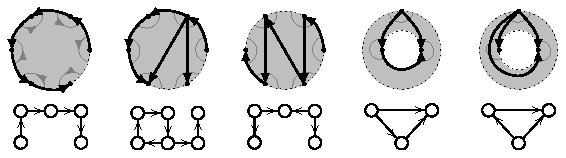
\includegraphics[width=0.89\textwidth]{figures/Fig_151_PDF265_Book253.pdf}
  \caption{生成弧系及其箭图（原书 p.253）}\label{fig:arc-collections-quivers}
\end{figure}
\end{example}

对每个弧系，其箭图都有一个特殊性质：每个顶点至多有两条入箭和两条出箭。因此，对每条箭 $\beta$，以 $\beta$ 开始的长度为 $2$ 的路径至多有两条。若路径 $\alpha\beta$ 中的两角在标记点周围的圆上相邻，就称它为角状路径\index{jiaozhuanglujing@角状路径|hyperpage}；若两角在多边形内相邻，则称它为面状路径\index{mianzhuanglujing@面状路径|hyperpage}。分别记角状路径集为 $P^+$（它们绕标记点逆时针转向）和面状路径集为 $P^-$（它们绕多边形顺时针转向）。

\begin{figure}[H]\centering
  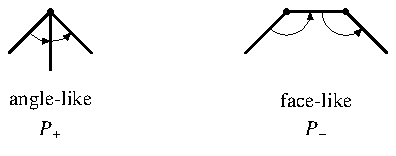
\includegraphics[width=0.48\textwidth]{figures/Fig_152_PDF265_Book253.pdf}
  \caption{角状路径与面状路径（原书 p.253）}\label{fig:angle-like-face-like}
\end{figure}

\begin{definition}{弧系的 gentle $A_\infty$ 代数}{gentle-a-infinity-algebra}\index{gentleadaishu@gentle $A_\infty$ 代数|hyperpage}
弧系的 gentle $A_\infty$ 代数是箭图 $Q_A$ 的路径代数除以面状路径所生成的理想：
\[
  \mathrm{Gtl}^{\pm}A:=\frac{\mathbb C Q_A}{\langle\alpha\beta\mid\alpha\beta\in P^-\rangle}.
\]
它的 $\mathbb Z_2$ 分次按下图规则赋予：
\begin{figure}[H]\centering
  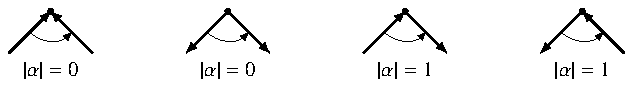
\includegraphics[width=0.65\textwidth]{figures/Fig_153_PDF265_Book253.pdf}
  \caption{弧系箭的 $\mathbb Z_2$ 次数（原书 p.253）}\label{fig:arc-degree-rule}
\end{figure}
在 $\mathrm{Gtl}^{\pm}A$ 上定义如下 $A_\infty$ 结构：若 $\beta_1,\ldots,\beta_l$ 是一个无内部标记点、边界由弧组成的浸入多边形上的连续各角，则
\[
  \mu(\alpha\beta_1,\beta_2,\ldots,\beta_k)=\alpha,
  \qquad
  \mu(\beta_1,\ldots,\beta_k\gamma)=(-1)^{|\gamma|}\gamma.
\]
% [Tutor Note: 定义正文说 $\beta_1,\ldots,\beta_l$ 是一个多边形的连续各角，两条乘积公式却写成 $\beta_k$；原书 p.253 此处指标不一致，按上下文两处应指同一组角，代入时以正文的 $\beta_l$ 为准。]
\end{definition}

\begin{figure}[H]\centering
  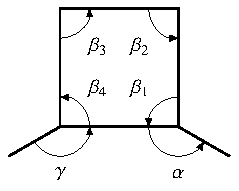
\includegraphics[width=0.44\textwidth]{figures/Fig_154_PDF266_Book254.pdf}
  \caption{高阶乘积的边界角（原书 p.254）}\label{fig:gentle-product-four-gon}
\end{figure}

\begin{lemma}{gentle 代数上的高阶乘积定义了 $A_\infty$ 结构}{gentle-algebra-ainfty-structure}
上述规则定义了一个 $A_\infty$ 结构\bookcite{115,36}。
\end{lemma}
\begin{proof}[证明思路]
首先，乘积的 $\mathbb Z_2$ 次数正确。若 $\alpha_1,\ldots,\alpha_k$ 位于某个多边形上，且所有弧沿多边形的方向一致，则所有 $\alpha_i$ 的次数都是 $1$。删去这些弧时，次数变化为 $k$；在 $\mathbb Z_2$ 中这与 $2-k$ 相同。若改变一条弧的方向，则有两个 $\alpha_i$ 的次数改变 $1$，总次数模 $2$ 不变。

下面验证 $A_\infty$ 关系。若
\[
\mu\bigl(\alpha_1,\ldots,\alpha_k,\mu(\alpha_{k+1},\ldots,\alpha_l),\ldots,\alpha_n\bigr)\ne0,
\]
根据内外两层乘积是否为二元乘积，可分为四种情形。
\begin{itemize}
  \item 若两者都是二元乘积，这就是普通乘积的结合律。
  \item 若外层乘积是二元乘积，则有
  \[
    \mu\bigl(\alpha_1,\mu(\alpha_2\beta_1,\ldots,\beta_k)\bigr)
    -\mu\bigl(\mu(\alpha_1,\alpha_2\beta_1),\ldots,\beta_k\bigr)=0.
  \]
  相应的两项来自同一多边形的两种分解：
  \begin{figure}[H]\centering
    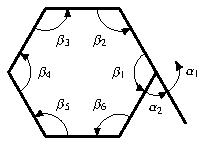
\includegraphics[width=0.42\textwidth]{figures/Fig_155_PDF266_Book254.pdf}
    \caption{外层乘积为二元乘积时的抵消（原书 p.254）}\label{fig:ainfty-cancellation-outer}
  \end{figure}
  \item 若内层乘积是二元乘积，则位于内层中间的弧把浸入多边形分成两个多边形，从而得到两个非零高阶乘积项，二者相消。
  \item 若内外两层都是高阶乘积，这两个多边形粘合成一个较大的浸入圆盘；相应地会出现一个内层为二元乘积的非零项，与原项相消：
  \begin{figure}[H]\centering
    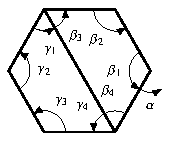
\includegraphics[width=0.48\textwidth]{figures/Fig_156_PDF266_Book254.pdf}
    \caption{两个高阶乘积对应的抵消项（原书 p.254）}\label{fig:ainfty-cancellation-higher}
  \end{figure}
  \[
    \mu(\alpha\beta_1,\beta_2,\mu(\beta_3\gamma_1,\gamma_2,\gamma_3,\gamma_4),\beta_4)
    -\mu(\alpha\beta_1,\beta_2,\beta_3\gamma_1,\gamma_2,\gamma_3,\mu(\gamma_4,\beta_4))=0.
  \]
\end{itemize}
每种情形中恰有两个非零项，并且它们互相抵消。\hfill$\square$
\end{proof}

\begin{lemma}{高阶乘积与有限维性}{gentle-algebra-finiteness}
设 $A$ 是剖分曲面的弧\index{poufenqumiandehu@剖分曲面的弧|hyperpage}系，$(\mathrm{Gtl}^{\pm}A,\mu)$ 是相应的 gentle $A_\infty$ 代数。
\begin{enumerate}[label=(\roman*)]
  \item 高阶乘积全为零，当且仅当不存在闭多边形。
  \item gentle 代数有限维，当且仅当不存在内部标记点。
\end{enumerate}
\end{lemma}
\begin{proof}[证明思路]
每个非零高阶乘积都来自一个边界由弧组成的浸入多边形。这样的多边形必由若干闭多边形粘合而成。gentle 代数中的非零路径对应标记点周围的角；若标记点在内部，这些角可以无限次地连续转绕。\hfill$\square$
\end{proof}
% [Tutor Note: 第一条的“当且仅当”要两边验证：若存在闭多边形，其各角按规则相乘得到 $\lambda\,1_a$（$\lambda\ne0$），故有非零高阶乘积；反之任何非零高阶乘积所在浸入多边形的边界都由闭多边形拼成。]

\begin{example}[含内部标记点的圆盘]
取一个圆盘，内部有 $k$ 个标记点，边界上有 $l$ 个标记点。把一个内部标记点连接到所有其他标记点。所得箭图是一个循环箭图；连接两个内部点的弧所对应的顶点上带有环。所有箭的次数均为 $0$，环与其他箭的乘积为零。该 gentle 代数是无限维的，但没有高阶乘积。
\begin{figure}[H]\centering
  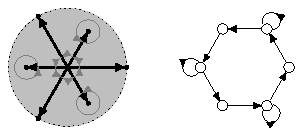
\includegraphics[width=0.43\textwidth]{figures/Fig_157_PDF267_Book255.pdf}
  % [Fig] 原书 p.255
\end{figure}
\end{example}

若考虑内圈和外圈各有 $k$ 个标记点的环带，可以用之字形弧将内外标记点相连。由此得到的循环箭图中箭的方向交替变化。此时没有关系，也没有高阶乘积，因此 gentle 代数就是路径代数。
\begin{figure}[H]\centering
  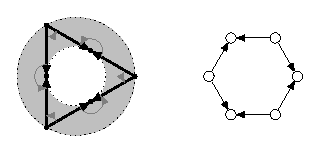
\includegraphics[width=0.43\textwidth]{figures/Fig_158_PDF267_Book255.pdf}
  % [Fig] 原书 p.255
\end{figure}

\begin{note}\label{note:gentle-algebra-classical}
gentle 代数最初由 Assem 和 Skowroński 在文献\bookcite{14}中引入，指满足下列条件的一类无分次路径代数 $\mathbb C Q/I$：
\begin{enumerate}[label=(G\arabic*)]
  \item $Q$ 没有有向环，且每个顶点至多有两条入箭和两条出箭；
  \item $I$ 由长度为 $2$ 的路径生成；
  \item 对每条箭 $\alpha\in Q_1$，至多有一条路径 $\alpha\beta$ 属于 $I$，也至多有一条路径 $\gamma\alpha$ 属于 $I$；
  \item 对每条箭 $\alpha$，至多有一条路径 $\alpha\beta$ 不属于 $I$，也至多有一条路径 $\gamma\alpha$ 不属于 $I$。
\end{enumerate}
引入这类代数，是因为它们具有良好的表示论性质，因而可以分类其不可分解表示。它们与镜像对称的联系则是后来才发现的\bookcite{3,36,115,166}。
\end{note}

\begin{theorem}{Lekili--Polishchuk 定理}{gentle-algebras-from-surfaces}
每个上述意义下的 gentle 代数都来自某个曲面。\bookcite{166}\footnote{这是 Lekili 与 Polishchuk 定理的一个特例；他们的结果处理的是 $\mathbb Z$ 分次版本。}
\end{theorem}
\begin{proof}[证明思路]
我们分步构造曲面。
\begin{enumerate}[label=(\roman*)]
  \item 考虑所有满足 $\alpha_i\alpha_{i+1}\in I$ 的最长序列 $\alpha_1\cdots\alpha_k$。对每个这样的序列取一个 $(k+2)$ 边形，并按 $h(\alpha_1),h(\alpha_2),\ldots,h(\alpha_k),t(\alpha_k)$ 给除最后一条边以外的边标记。将箭画成沿多边形角落排列的小角。由 (G3)，每条箭恰好属于一个多边形。
  \item 考虑所有满足 $\beta_i\beta_{i+1}\notin I$ 的最长序列 $\beta_1\cdots\beta_k$。对每个这样的序列取一个标记点 $m_i$，并把每个多边形的角标为包含该角的序列所对应的标记点。
  \item 沿着具有相同标记的边与角粘合多边形。所得曲面可定向，因为各多边形上的角均顺时针排列，而标记点周围的角均逆时针排列。
  \item 定向各条边，使每个标记点处的边要么全部指向该点，要么全部从该点指出。
\end{enumerate}
这样得到一个弧系，它把曲面剖分为开多边形。相应的 gentle $A_\infty$ 代数集中在次数 $0$，没有高阶乘积，并且同构于 $\mathbb C Q/I$。\hfill$\square$
\end{proof}

\begin{theorem}{生成弧系改变时的拟等价}{gentle-derived-invariance}
同一带标记曲面的两个生成弧系所对应的 gentle $A_\infty$ 代数，其扭曲完备化彼此 $A_\infty$ 拟等价\bookcite{115,36}。
\end{theorem}
\begin{proof}[证明思路]
若 $A'$ 是把弧 $a$ 的方向反转后由 $A$ 得到的，则可以把 $\mathrm{Gtl}^{\pm}A'$ 嵌入 $\mathrm{TwGtl}^{\pm}A$，方法是把反向弧识别为对象 $a[1]$（注意，$a$ 是 $Q_A$ 的顶点，因而也是范畴 $\mathrm{Gtl}^{\pm}A$ 的对象）。

若 $A$ 与 $A'=A\cup\{a\}$ 都是剖分曲面的弧系，则 $a$ 位于 $A$ 的某个多边形内，并可找到一列弧 $a_1,\ldots,a_k$，其首尾相接后可同位变形为 $a$：
\begin{figure}[H]\centering
  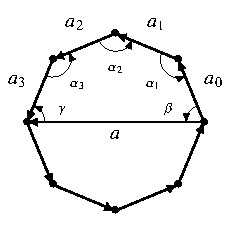
\includegraphics[width=0.62\textwidth]{figures/Fig_159_PDF269_Book257.pdf}
  \caption{把新增弧表示为扭曲复形（原书 p.257）}\label{fig:added-arc-twisted-complex}
\end{figure}
在范畴 $\mathrm{TwGtl}^{\pm}A'$ 中，对象 $a$ 与下列对象拟同构：
\[
  M=(a_0\oplus\cdots\oplus a_k,\alpha_1+\cdots+\alpha_k).
\]
事实上，设 $\beta$ 是 $a_0$ 与 $a$ 之间的角，$\gamma$ 是 $a$ 与 $a_k$ 之间的角，则 $\beta\in\mathrm{TwGtl}^{\pm}A'(M,a)$、$\gamma\in\mathrm{TwGtl}^{\pm}A'(a,M)$ 互为逆元，因为
\[
  \widehat\mu_2(\beta,\gamma)=\mu(\beta,\alpha_0,\ldots,\alpha_k,\gamma)=1_a,
\]
\[
  \widehat\mu_2(\gamma,\beta)=\sum_i\mu(\alpha_i,\ldots,\alpha_k,\gamma,\beta,\alpha_0,\ldots,\alpha_{i-1})
  =1_{a_1}+\cdots+1_{a_k}=1_M.
\]
因此，$\mathrm{Gtl}^{\pm}A$ 生成 $\mathrm{TwGtl}^{\pm}A'$。

只要两组弧都剖分曲面，添加或删除一条弧就不会改变扭曲完备化。不断添加弧，可将任一弧系扩充为曲面的三角剖分。Hatcher 定理\bookcite{110}说明，任意两个三角剖分都可以通过四边形中翻转对角线的操作互相转化（即删去一条对角线并以另一条替代）。
\begin{figure}[H]\centering
  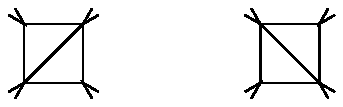
\includegraphics[width=0.36\textwidth]{figures/Fig_160_PDF269_Book257.pdf}
  \caption{翻转四边形的对角线（原书 p.257）}\label{fig:flip-diagonal}
\end{figure}
由此即可得到结论。\hfill$\square$
\end{proof}

\begin{definition}{带标记曲面的拓扑 Fukaya 范畴}{topological-fukaya-marked-surface}
带标记曲面 $(S,M)$ 的 $\mathbb Z_2$ 分次拓扑 Fukaya 范畴\index{tuopufukayafanchou@拓扑 Fukaya 范畴|hyperpage}，定义为任一剖分弧系 $A$ 所对应的 gentle $A_\infty$ 范畴的导出范畴：
\[
  \mathrm{topFuk}^{\pm}(S,M):=D\mathrm{Gtl}^{\pm}A.
\]
\end{definition}

\begin{example}[三类经典箭图]
第四章研究过的线性箭图、Kronecker 箭图和循环箭图，都属于这一框架。它们的导出范畴分别等价于下列带标记曲面的拓扑 Fukaya 范畴：边界上有 $n$ 个标记点的圆盘；两个边界分支上各有一个标记点的圆柱；内部有一个标记点、边界上有 $n$ 个标记点的圆盘。
\end{example}

\begin{note}\label{note:marked-surface-conventions}
文献中对带标记曲面有不同约定，差异在于如何处理标记点和边界分支：
\begin{enumerate}[label=(\roman*)]
  \item 文献\bookcite{3,156,36}采用与本书相同的约定。
  \item 在文献\bookcite{115}中，标记点被切除。内部标记点变成一个小的标记边界圆；带有 $n$ 个标记点的边界分支变成由 $2n$ 段组成的边界，标记段和非标记段交替排列。弧的端点落在标记边界段上；不同弧的端点彼此不同（但可以落在同一标记段上），角则是这些标记边界段的子段。角也称为 Reeb 弦。
  \item 在文献\bookcite{166}中，边界的非标记段被压缩成点，并称作 stop（文献中有时也管它叫标记点，容易混淆），因为它们会阻碍 Reeb 弦的流动。
  \item 在文献\bookcite{204}中，采用带状图的对偶形式（见定义\ref{def:ribbon-graph}）。每个多边形的中心成为带状图的一个节点，并与多边形的各边相连，构成带状图的半边。
\end{enumerate}
\begin{figure}[H]\centering
  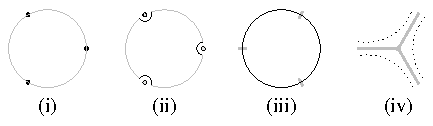
\includegraphics[width=0.9\textwidth]{figures/Fig_161_PDF270_Book258.pdf}
  \caption{四种带标记曲面的约定（原书 p.258）}\label{fig:marked-surface-conventions}
\end{figure}
\end{note}

\begin{note}\label{note:marked-surface-generalizations}
带标记曲面的概念还有一些有时很有用的推广。
\begin{itemize}
  \item \textbf{同位变形的弧。}若弧 $a,b$ 可以通过同位变形互相变换，则它们围成一个二边形。若把高阶乘积规则扩展到二边形，就会得到 $\mu_2(\alpha,\beta)=\pm1_a$ 和 $\mu_2(\beta,\alpha)=\pm1_b$，因此 $a,b$ 是同构对象。含有 $a,b$ 两条弧的集合严格说来不再给出 gentle 代数，但所得代数与只含 $a$ 的 gentle 代数 Morita 等价。二边形见图\ref{fig:isotopic-arcs-digon}。
  \begin{figure}[H]\centering
    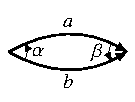
\includegraphics[width=0.18\textwidth]{figures/Fig_162_PDF271_Book259.pdf}
    \caption{同位变形的弧围成二边形（原书 p.259）}\label{fig:isotopic-arcs-digon}
  \end{figure}
  \item \textbf{曲面中的穿孔。}可以把穿孔建模为 $S\setminus M$ 内部的另一组点 $P$。弧不得经过这些点，也不得以它们为端点；生成弧系的每个多边形至多包含一个穿孔。定义高阶乘积时，只考虑不覆盖穿孔的浸入多边形。
  \item \textbf{轨形点。}可以把轨形点建模为 $S\setminus M$ 内部的点 $o_i$，并给每个点赋予次数 $d_i\ge2$。弧不得经过这些点，也不得以它们为端点；生成弧系的每个多边形至多包含一个轨形点。若多边形含有次数为 $d_i$ 的轨形点，则要求
  \[
    \mu(\underbrace{\beta_1,\ldots,\beta_k,\ldots,\beta_1,\ldots,\beta_k}_{d_i\text{ 次}})=h(\beta_1),
  \]
  其中 $\beta_1,\ldots,\beta_k$ 是该多边形的各角。其他乘积可以通过提升到轨形万有覆盖来计算。
  \item \textbf{面积。}若给每个多边形赋予面积，则可以用因子 $e^{-A}$ 对高阶乘积 $\mu$ 加权，其中 $A$ 是浸入多边形的总面积。通常可通过 gentle 代数的自同构消去这些面积参数。
\end{itemize}
\end{note}

\section{从弧到弦与带}\label{sec:arcs-strings-bands}
\takeaway{把首尾相接的弧用角缝合，开曲线实现为扭曲复形上的弦对象，闭曲线实现为带局部系统的带对象；交点是态射，曲线围成的多边形计数高阶乘积，故 $\mathrm{topFuk}^{\pm}$ 可看作 Fukaya 范畴的组合模型。}
称 $\mathrm{topFuk}^{\pm}(S,M)$ 为拓扑 Fukaya 范畴，是因为其中的对象可以与曲面上开曲线和闭曲线的同伦类对应。本节将说明如何把这类对象构造为 gentle $A_\infty$ 代数上的扭曲复形。更多细节见\bookcite{115,36,37}。

考虑一列弧 $a_1[i_1],\ldots,a_k[i_k]$，其中各弧经过平移后首尾相接。对每对相邻弧 $a_u[i_u]$ 与 $a_{u+1}[i_{u+1}]$，选取一个绕公共标记点的角 $\alpha_u$；它可以从 $a_u$ 指向 $a_{u+1}$，也可以反向。注意，$\alpha_u$ 可视为 $a_u[i_u]$ 到 $a_{u+1}[i_{u+1}]$ 或反向的次数为 $1$ 的态射。由此可定义两个对象：
\begin{itemize}
  \item 在曲面 $S$ 上，用沿角 $\alpha_u$ 的小弦把各弧缝合，得到浸入曲线 $L$；
  \item 在 $\mathrm{TwGtl}^{\pm}A$ 中定义复形
  \[
    (L,\delta):=\left(\bigoplus_{j=1}^k a_j[i_j],\ \sum_{u=1}^{k-1}\alpha_u\right).
  \]
\end{itemize}
曲线 $L$ 的几何性质与相应扭曲复形的代数性质紧密相关。
\begin{figure}[H]\centering
  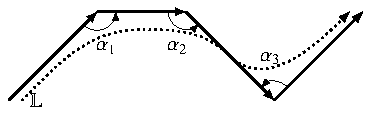
\includegraphics[width=0.52\textwidth]{figures/Fig_163_PDF272_Book260.pdf}
  \caption{用弧与角拼接出曲线及其扭曲复形（原书 p.260）}\label{fig:string-from-arcs}
\end{figure}

\begin{lemma}{开弦对象的基本性质}{string-object-properties}
设 $L$ 是一条曲线，$(L,\delta)$ 是与之对应的扭曲复形。
\begin{enumerate}[label=(\roman*)]
  \item $(L,\delta)$ 满足 Maurer--Cartan 方程，当且仅当 $L$ 不含在 $S\setminus M$ 中可缩的环；
  \item 与彼此同位变形的曲线对应的扭曲复形在 $\mathrm{topFuk}^{\pm}(S,M)$ 中同构；
  \item 对每个同伦类，都存在一列弧，使其缝合得到属于该同伦类的曲线 $L$。
\end{enumerate}
\end{lemma}
\begin{proof}[证明思路]
若存在可缩环，则环内各角 $\alpha_u$ 会给出非零乘积 $\mu(\alpha_u,\ldots,\alpha_v)$。若不存在可缩环，则 Maurer--Cartan 方程中的所有高阶乘积均为零。普通乘积也全为零：扭曲微分 $\delta$ 中相邻的两个角要么不可复合，要么其乘积由 gentle 代数中的关系置零。
相邻角的两种情形如下：
\begin{figure}[H]\centering
  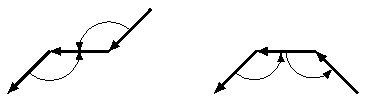
\includegraphics[width=0.5\textwidth]{figures/Fig_164_PDF272_Book260.pdf}
  \caption{相邻角的乘积为零的两种情形（原书 p.260）}\label{fig:consecutive-string-angles}
\end{figure}

为证第二条，考虑两列只在某一个多边形处不同的弧序列：一列沿多边形顺时针绕行，另一列沿逆时针绕行。由此得到扭曲对象 $(L_1,\delta_1)$ 与 $(L_2,\delta_2)$。令 $u=\sum 1_a+\beta_1\in\mathrm{Hom}^{\bullet}(L_1,L_2)$、$v=\sum 1_a+\beta_2\in\mathrm{Hom}^{\bullet}(L_2,L_1)$，其中求和遍历 $L_1,L_2$ 的公共箭。计算扭曲乘积时，插入多边形各角会产生额外的高阶乘积项；结果为
\[
\begin{aligned}
\widehat\mu(u,v)
&=\sum_{a\in L_1\cap L_2}1_a+
\sum\mu\bigl(\cdots\alpha_i^{L_2}\cdots,\beta_1,
\cdots\alpha_i^{L_1}\cdots,\beta_2,\cdots\alpha_i^{L_2}\cdots\bigr)\\
&=\sum_{a\in L_1\cap L_2}1_a+
\sum_{a\in L_2\setminus L_1}1_a=1_{L_2}.
\end{aligned}
\]
反向乘积同理，因此 $u,v$ 互为逆元。两条彼此同位变形的曲线之间的局部变换如下：
\begin{figure}[H]\centering
  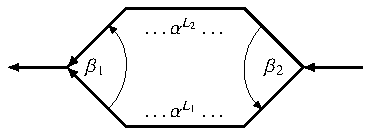
\includegraphics[width=0.52\textwidth]{figures/Fig_165_PDF273_Book261.pdf}
  \caption{在多边形内改变弧的绕行方向（原书 p.261）}\label{fig:isotopy-string-curves}
\end{figure}
任意两条彼此同位变形的曲线都可以通过一系列这类局部变换互相得到。

为证第三条，先对曲线作同位变形，使其不含可缩环；再把曲线每次穿过多边形的线段替换为沿多边形顺时针或逆时针绕行的弧序列，并用多边形内的角把各箭缝合起来。\hfill$\square$
\end{proof}

\begin{definition}{弦对象}{string-object}
连接两个标记点的曲线 $L$ 所对应的弦对象\index{xianduixiang@弦对象|hyperpage} $S(L)$，是由一列近似该曲线的弧所得到的扭曲对象 $(L,\delta)$。
\end{definition}

\begin{lemma}{弦对象的自同态空间}{string-object-endomorphisms}
设 $a$ 是连接两个不同标记点 $p_1,p_2$ 的弧。
\begin{enumerate}[label=(\roman*)]
  \item 若 $p_1,p_2$ 都是内部点，则
  \[
    \mathrm{topFuk}^{\pm}(S(a),S(a))\cong k[\ell_1,\ell_2]/(\ell_1\ell_2).
  \]
  \item 若只有 $p_1$ 是内部点，则 $\mathrm{topFuk}^{\pm}(S(a),S(a))\cong k[\ell_1]$。
  \item 若 $p_1,p_2$ 都在边界上，则 $\mathrm{topFuk}^{\pm}(S(a),S(a))\cong k$。
\end{enumerate}
\end{lemma}
\begin{proof}[证明思路]
取一个包含 $a$ 的弧系，并构造 gentle 代数 $\mathrm{Gtl}^{\pm}A$。第一种情形下，
\[
  \mathrm{topFuk}^{\pm}(S(a),S(a))=1_a\cdot\mathrm{Gtl}^{\pm}A\cdot1_a.
\]
这个空间由所有从 $e_a$ 出发的非零环路张成。基本环路有两个：$\ell_1$ 绕过 $a$ 的头端，$\ell_2$ 绕过尾端；它们的乘积由 gentle 代数中的关系置零。其余情形类似。
\begin{figure}[H]\centering
  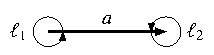
\includegraphics[width=0.42\textwidth]{figures/Fig_166_PDF273_Book261.pdf}
  \caption{弧两端的基本环路（原书 p.261）}\label{fig:string-end-loops}
\end{figure}
\hfill$\square$
\end{proof}

闭曲线也能构造出对象。先取一列首尾相接成环的弧 $a_1[i_1],\ldots,a_k[i_k]$，再用角 $\alpha_u$ 缝合它们，得到闭曲线 $L$。此时还需一个角 $\alpha_k$ 连接 $a_k$ 与 $a_1$。图中画出由此得到的曲线：
\begin{figure}[H]\centering
  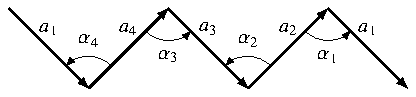
\includegraphics[width=0.52\textwidth]{figures/Fig_167_PDF275_Book263.pdf}
  \caption{用弧与角拼接闭曲线（原书 p.263）}\label{fig:closed-curve-from-arcs}
\end{figure}
选取映射 $\lambda\colon\{1,\ldots,k\}\to\mathrm{GL}_n(k)$，并定义
\[
  (L,\delta):=\left(\bigoplus_{j=1}^k a_j[i_j]^{\oplus n},\ \sum_{u=1}^k\lambda_u\alpha_u\right).
\]
定义沿曲线的绕行变换（holonomy）$T^\lambda$ 为各个 $\lambda_i^{\pm1}$ 的乘积：若 $\alpha_u$ 的转向与 $L$ 一致，指数取 $+1$；若方向相反，则取 $-1$。

\begin{lemma}{带绕行变换的闭曲线对象}{band-object-properties}
设 $L$ 是一条曲线，$\lambda\colon\{1,\ldots,k\}\to\mathrm{GL}_n(k)$，$(L,\delta)$ 是相应扭曲复形。
\begin{enumerate}[label=(\roman*)]
  \item 矩阵 $\delta$ 为下三角矩阵，当且仅当 $T^\lambda$ 的各因子指数不全相同。
  \item $\delta$ 满足 Maurer--Cartan 方程，当且仅当 $L$ 不含可缩环。
  \item 对应于彼此同位变形的曲线、且绕行变换共轭的两对数据，给出 $\mathrm{topFuk}^{\pm}(S,M)$ 中同构的对象。
  \item 对每个同伦类，都可以找到一列弧，使其缝合曲线 $L$ 属于该同伦类。
\end{enumerate}
\end{lemma}
\begin{proof}[证明思路]
第一条由下述观察得到：所有指数相同，当且仅当 $\alpha_i$ 在 $Q_A$ 中构成一个有向环。第二条和第四条的证明与弦对象相同。为证第三条，若 $L$ 的各段上有矩阵 $G_i\in\mathrm{GL}_n(k)$，可取
\[
  G=\sum_j G_j\otimes1_{a_j},\qquad G^{-1}=\sum_j G_j^{-1}\otimes1_{a_j}.
\]
若 $\lambda_i'=G_{i-1}\lambda_iG_i^{-1}$，则
\[
  (dG)_j=\lambda_j'G_j-G_{j-1}\lambda_j=0.
\]
因此
\[
G\in H\mathrm{Hom}^{\bullet}\left(
  \bigoplus_{j=1}^k a_j[i_j]^{\oplus n},
  \bigoplus_{j=1}^k a_j[i_j]^{\oplus n}
\right)
=\mathrm{topFuk}^{\pm}\bigl((L,\delta_\lambda),(L,\delta_{\lambda'})\bigr)
\]
是两扭曲对象之间的同构，并且 $T^{\lambda'}=G_1T^\lambda G_1^{-1}$。\hfill$\square$
\end{proof}
% [Tutor Note: 下标至关重要：$\lambda_i'=G_{i-1}\lambda_iG_i^{-1}$ 中左乘的 $G_{i-1}$ 与右乘的 $G_i^{-1}$ 来自沿曲线搬运矩阵指标时的同一次平移，但位置相反；代入 $(dG)_j=\lambda_j'G_j-G_{j-1}\lambda_j$ 后绕一圈，中间项两两相消，剩下的正是共轭 $T^{\lambda'}=G_1T^{\lambda}G_1^{-1}$，与引理第三条“绕行变换共轭”对应。]

\begin{definition}{带对象}{band-object}
扭曲对象 $(L,\delta)$ 称为与 $(L,T^\lambda)$ 对应的带对象\index{daiduixiang@带对象|hyperpage}。记为 $B(L,T^\lambda)$，以强调它只依赖曲线的同伦类和绕行变换的共轭类。
\end{definition}

\begin{note}\label{note:bands-local-systems}
从几何上看，$(L,T^\lambda)$ 可以视为带有局部系统的曲线。也可以给弦对象引入局部系统，但此时可以通过基变换把所有 $\lambda$ 矩阵化为恒等矩阵，因而扭曲对象就是 $n$ 个弦对象的直和。开曲线的基本群平凡，所以其上的局部系统只有平凡者。

若一条带对象对应的曲线沿同一轨迹绕行 $l$ 次，且绕行变换为 $T^\lambda$，则也可以把它看成只绕行一次、但绕行变换为 $T^\lambda\otimes P$ 的带对象，其中 $P$ 是循环置换矩阵。
\end{note}

\begin{lemma}{简单闭曲线上带对象的态射}{band-self-homs}
设 $L$ 是简单闭曲线，$\lambda,\lambda'\in k^*$。则
\[
  \mathrm{topFuk}^{\pm}(B(L,\lambda),B(L,\lambda'))\cong
  \begin{cases}
    k\iota\oplus k\iota^*,&\lambda=\lambda',\\
    0,&\lambda\ne\lambda',
  \end{cases}
\]
其中 $\iota=1_B$ 是恒等态射，$\iota^*$ 的次数为 $1$。
\end{lemma}
\begin{proof}[证明思路]
选取弧系，使 $L$ 同位变形到一条连接角方向交替的弧路（即相邻角不可复合）。构造一条与 $L$ 同伦的路径，并令
\[
  B=\left(\bigoplus_{j=1}^k a_j,\ \delta=\sum_{j=1}^k\lambda_j\alpha_j\right),
\]
其中 $\alpha_j$ 是 $a_j$ 与 $a_{j+1}$ 之间的角，指标按模 $k$ 计算。为简便起见，先假设所有标记点都在边界上；含内部标记点的情形类似，但计算稍繁。此时
\[
  \mathrm{Hom}^{\bullet}(B,B)=\bigoplus_j k1_{a_j}+k\alpha_j,
\]
微分由交换子给出，因为不会出现更高阶乘积：
\[
  dx=\left[\sum_{j=1}^k\lambda_j\alpha_j,x\right].
\]
直接计算可知，其上同调由 $\iota=1_B=\sum_a1_a$ 和 $\iota^*=\lambda_j\alpha_j$ 张成。第二个上同调类可取任一 $\lambda_j\alpha_j$，因为在上同调中它们至多相差一个倍数；具体而言，$d1_{a_j}=\pm(\lambda_j\alpha_j-\lambda_{j-1}\alpha_{j-1})$。若 $\lambda\ne\lambda'$，则 $d1_B\ne0$，而各个 $d1_{a_j}$ 的线性组合可消去某个 $\alpha_u$ 的倍数，故上同调为零。\hfill$\square$
\end{proof}

接下来考察两个不同带对象之间的态射。设 $L_1,L_2$ 是曲面 $S$ 上两条无自交闭曲线，且它们恰有一个交点 $p$。令 $B_1=B(L_1,\lambda_1)$、$B_2=B(L_2,\lambda_2)$ 是相应的带对象。取弧系，使交点 $p$ 落在一条弧上，并使该弧的定向与曲线方向一致；局部图形如下，且两曲线没有其他重叠：
\begin{figure}[H]\centering
  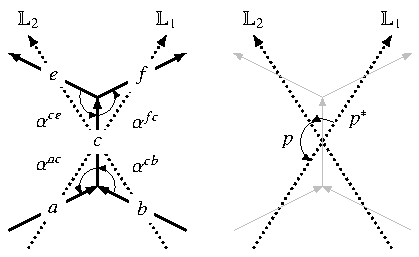
\includegraphics[width=0.56\textwidth]{figures/Fig_168_PDF276_Book264.pdf}
  \caption{两条闭曲线的局部交叉与相应角（原书 p.264）}\label{fig:band-intersection-local}
\end{figure}
于是
\[
  B_1=(a\oplus c\oplus f\oplus\cdots,\lambda_1^{ac}\alpha_{ac}+\lambda_1^{fc}\alpha_{fc}+\cdots),
\]
\[
  B_2=(b\oplus c\oplus e\oplus\cdots,\lambda_2^{cb}\alpha_{cb}+\lambda_2^{ce}\alpha_{ce}+\cdots),
\]
其中 $\alpha_{ac}$ 表示围绕公共标记点从 $c$ 指向 $a$ 的逆时针角。

\begin{lemma}{单个交点产生的带对象态射}{band-intersection-morphisms}
若两条曲线恰在一点 $p$ 相交，且 $B_1,B_2$ 是相应的一维局部系统带对象，则
\[
  \mathrm{topFuk}^{\pm}(B_1,B_2)=kp^*\oplus0,
  \qquad
  \mathrm{topFuk}^{\pm}(B_2,B_1)=0\oplus kp,
\]
其中 $p^*=1_c$，而 $p=\lambda_1^{ac}\alpha_{ac}-\lambda_2^{cb}\alpha_{cb}$。
\end{lemma}
\begin{proof}[证明思路]
仍假设所有标记点都在边界上。此时态射复形为
\[
  \mathrm{Hom}(B_1,B_2)=k1_c+k\alpha_{ba}+k\alpha_{ca}+k\alpha_{bc}+k\alpha_{ef}+k\alpha_{cf}+k\alpha_{ec},
\]
其微分为
\[
  x\longmapsto(\lambda_2^{cb}\alpha_{cb}+\lambda_2^{ce}\alpha_{ce})x
  -x(\lambda_1^{ac}\alpha_{ac}+\lambda_1^{fc}\alpha_{fc}).
\]
因此 $1_c$ 属于零次上同调；把它记为 $p$，因为它对应交点。容易验证，这就是唯一的上同调类。反向的态射空间中也有一个上同调类：$\lambda_1^{ac}\alpha_{ac}-\lambda_2^{cb}\alpha_{cb}$；也可以写成 $\lambda_1^{fc}\alpha_{fc}-\lambda_2^{ce}\alpha_{ce}$，因为两者之和是 $d1_c$。取前者记为 $p^*$，其次数为 $1$。\hfill$\square$
\end{proof}
% [Tutor Note: 证明把 $1_c$ 记作 $p$、把 $\lambda_1^{ac}\alpha_{ac}-\lambda_2^{cb}\alpha_{cb}$ 记作 $p^*$，与原书引理 9.24 的命名（$p^*=1_c$，$p=\lambda_1^{ac}\alpha_{ac}-\lambda_2^{cb}\alpha_{cb}$）正好相反；原书 p.264 亦如此。按下一引理的 $p\cdot p^*=\iota^*_{B_1}$ 与“后者次数为 $1$”，应以引理的命名为准，即 $1_c$ 是零次的 $p^*$。]

\begin{note}\label{note:multiple-band-intersections}
上述引理可以推广到有多个交点的曲线。每个交点都会在两个方向上各贡献一个态射，而态射的次数由两条曲线的定向决定。
\end{note}

\begin{lemma}{交点态射的乘积}{band-intersection-products}
若 $p$ 是两个带对象 $B_1,B_2$ 的交点，则
\[
  p\cdot p^*=\iota_{B_1}^*,\qquad p^*\cdot p=-\iota_{B_2}^*.
\]
\end{lemma}
\begin{proof}[证明思路]
这直接由 $\iota,\iota^*,p,p^*$ 的定义得到。\hfill$\square$
\end{proof}

现在设闭曲线 $L_1,\ldots,L_k$ 围成 $\dot S$ 中的一个多边形区域，并且存在弧系，使局部图形如下。把从 $L_{i+1}$ 到 $L_i$ 的次数 $1$ 态射记作 $p_i$，反方向的次数 $0$ 态射记作 $p_i^*$。
\begin{figure}[H]\centering
  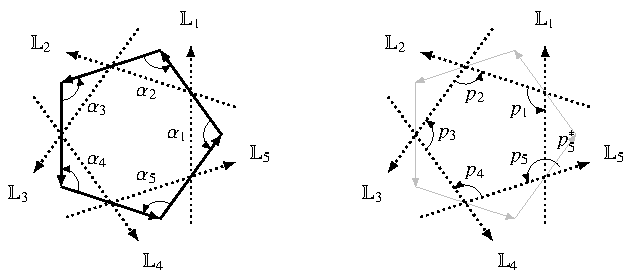
\includegraphics[width=0.66\textwidth]{figures/Fig_169_PDF277_Book265.pdf}
  \caption{由闭曲线围成的多边形区域（原书 p.265）}\label{fig:band-polygon-products}
\end{figure}

\begin{lemma}{多边形上的高阶乘积}{band-higher-product-polygon}
在上述情形中，
\[
  \mu(p_1,\ldots,p_{k-1})=c\,p_k^*,
  \qquad c=\lambda_1\cdots\lambda_k,
\]
其中 $c$ 是沿闭路的绕行变换。
\end{lemma}
\begin{proof}[证明思路]
每个 $p_i$ 的表达式形如 $\lambda_i\alpha_i+\cdots$，其中省略项是多边形外部的角，在计算中不起作用。带对象 $B(L_i,\lambda_i)$ 的扭曲微分也形如 $\lambda_i\alpha_i+\cdots$（以 $\lambda_i$ 表示角 $\alpha_i$ 上的系数）。计算 $\mu(p_1,\ldots,p_{k-1})$ 时，需要在各态射之间以所有可能方式插入 $\delta_i$ 并求和。唯一可能的非零乘积，是把 $\delta_k$ 插在末尾：
\[
  \mu(\lambda_1\alpha_1+\cdots,\ldots,\lambda_{k-1}\alpha_{k-1}+\cdots,
  \lambda_k\alpha_k+\cdots)=\lambda_1\cdots\lambda_k1_{a_k}.
\]
这是第 $k$ 条弧的恒等态射，对应于 $c p_k^*\in\mathrm{topFuk}^{\pm}(B_1,B_k)$。这项计算尚未在极小模型中进行；转入极小模型后结果仍然相同，因为其他可能贡献的树都会包含为零的乘积 $\mu_2(\alpha_i,\alpha_{i+1})$。\hfill$\square$
\end{proof}

与这个多边形对应的另一个乘积则依赖于所选的极小模型。为了在极小模型中计算乘积，对每个带对象 $B=(\bigoplus_i a_i,\lambda_i\alpha_i)$，需要选取分解
\[
  \mathrm{Hom}^{\bullet}(B,B)=I^{\bullet}\oplus H^{\bullet}\oplus R^{\bullet}.
\]
为此，选取一条弧 $a_m$ 和一个角 $\alpha_m$，称为标记弧和标记角。零次部分中，把除 $1_{a_m}$ 外的所有 $1_a$ 放入 $R^0$，并把 $1_B$ 放入 $H^0$；一次部分中，把 $\lambda_m\alpha_m$ 放入 $H^1$，并把所有 $\lambda_i\alpha_i-\lambda_{i+1}\alpha_{i+1}$ 放入 $I^1$。

\begin{lemma}{依赖标记弧的极小模型乘积}{minimal-model-polygon-product}
在上述情形中，
\[
  \mu(p_1,\ldots,p_{k-1},p_k)=c1_{L_k}\quad\text{或}\quad0.
\]
当且仅当 $L_k$ 的标记弧属于该多边形时，乘积取第一种情形。
\end{lemma}
\begin{proof}[证明思路]
此时唯一可能的非零乘积，是不插入任何 $\delta_i$ 的项：
\[
  \mu(\lambda_1\alpha_1+\cdots,\ldots,\lambda_k\alpha_k+\cdots)
  =\lambda_1\cdots\lambda_k1_{a_k}=c1_{a_k}.
\]
但 $1_{a_k}$ 不是 $\mathrm{Hom}(B(L_k,\lambda),B(L_k,\lambda))$ 中的上同调类，因此转到极小模型时须投影到上同调。该自同态空间中的零次上同调类为 $1_{L_k}=\sum_{a\in L_k}1_a$。由于除 $1_{a_m}$ 外的所有 $1_a$ 都被放在 $R$ 中，相应投影把它们映为零，并把 $1_{a_m}$ 映为 $1_{L_k}$。\hfill$\square$
\end{proof}

\begin{note}\label{note:geometric-fukaya-product}
这种现象与 Fukaya 范畴的几何构造相似。为了定义一条拉格朗日子流形与自身之间的态射空间，必须先选取一个变形。变形曲线与原曲线相交于两点，其中一点对应恒等态射。若这一点落在多边形边界上，就会有非零乘积；若落在多边形之外，则没有贡献。下图给出两种情形：
\begin{figure}[H]\centering
  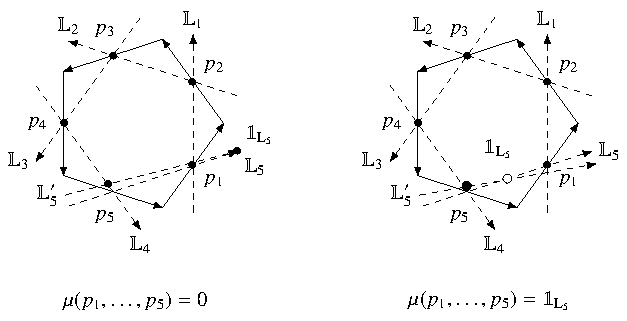
\includegraphics[width=0.89\textwidth]{figures/Fig_170_PDF279_Book267.pdf}
  \caption{多边形乘积的两种情形（原书 p.267）}\label{fig:polygon-products-two-cases}
\end{figure}
还需注意，上述乘积并非全部非零乘积。要完整计算所有乘积，技术上十分繁复，本书不再尝试。
\end{note}

由前述引理可知，带对象之间的态射由交点给出，而这些交点态射的乘积则通过计数由曲线围成的浸入圆盘得到。这正是我们对 Fukaya 型范畴所预期的行为。因此，可以把 $\mathrm{topFuk}^{\pm}(S,M)$ 看作 Fukaya 范畴的一种代数定义的替代模型。给定带标记曲面 $(S,M)$，可以构造一个带柱形端和 stop 的 Liouville 流形 $(X,\sigma)$：
\begin{enumerate}[label=(\roman*)]
  \item 在每个内部标记点周围切去一个圆盘。所得带边界曲面可赋予 Liouville 域 $X_0$ 的结构；
  \item 在由内部标记点产生的边界上粘接不带 stop 的圆柱；
  \item 对每个带有 $k$ 个标记点的边界分支，粘接带有 $k$ 个 stop 的圆柱。这些 stop 是终止在相邻标记点之间边界上的曲线。
\end{enumerate}

\begin{theorem}{拓扑 Fukaya 范畴与 partially wrapped Fukaya 范畴}{topological-partially-wrapped-equivalence}
带标记曲面 $(S,M)$ 的 Fukaya 范畴与 $(X,\sigma)$ 的 partially wrapped Fukaya 范畴 $A_\infty$ 等价：
\[
  \mathrm{topFuk}^{\pm}(S,M)\cong_\infty\mathrm{wrFuk}^{\pm}_{\sigma}X.
\]
\end{theorem}
\begin{proof}[证明思路]
在标记点附近把每条弧延伸到无穷远，可把它变成具有锥形端的拉格朗日子流形。在 partially wrapped Fukaya 范畴中，这些拉格朗日子流形之间的态射空间与 $\mathrm{topFuk}^{\pm}(S,M)$ 中弧之间的态射空间相同，因为每一次 Reeb 流动都对应一个角。两侧的高阶乘积也一致，因为浸入圆盘恰好对应于曲面 $S$ 上的多边形。最后，由于弧系把曲面剖分为多边形，可以应用定理\ref{thm:abouzaid-generation-criterion}中的生成判据，证明这些带锥形端的拉格朗日子流形生成 Fukaya 范畴。更多细节见文献\bookcite{36}的附录。\hfill$\square$
\end{proof}

在上述对应中，弦对象对应开拉格朗日子流形，带对象对应带局部系统的闭拉格朗日子流形。因此，可以把带标记曲面的（部分）wrapped Fukaya 范畴定义为由弦对象生成的范畴，而把正合 Fukaya 范畴定义为由带对象生成的子范畴：
\[
\begin{aligned}
  \mathrm{wrFuk}^{\pm}(S,M)&:=\langle S(L)\mid S(L)\text{ 是弦对象}\rangle
  =\mathrm{topFuk}^{\pm}(S,M),\\
  \mathrm{exFuk}^{\pm}(S,M)&:=\langle B(L,\lambda)\mid B(L,\lambda)\text{ 是带对象}\rangle
  \subset\mathrm{topFuk}^{\pm}(S,M).
\end{aligned}
\]

\begin{note}\label{note:exact-fukaya-spin-morse}
传统上，正合 Fukaya 范畴的对象是带有自旋结构和 Morse 函数的闭曲线\bookcite{218}。自旋结构用于确定符号；Morse 函数则用来定义 $L$ 的自同态，把曲线与其在该 Morse 函数下的 Hamilton 变形的交点视为态射。可以在曲线 $L$ 上标出三个特殊点 $\circ,*,\times$ 来表示这些数据。
\begin{itemize}
  \item $\circ$ 是 Morse 函数的极小点，对应 $\iota=1_L$。在本书的设定中，这等价于选择标记弧，并把 $\circ$ 放在标记弧之前；
  \item $*$ 是 Morse 函数的极大点，对应 $\iota^*=\lambda_m\alpha_m$。在本书的设定中，这等价于选择标记角，并把 $*$ 放在对应于 $\alpha_m$ 的线段中间；
  \item $\times$ 是自旋结构发生翻转的位置。在本书的术语中，带非平凡自旋结构的曲线具有绕行变换为 $-1$ 的局部系统。这可以通过令除一个以外的所有 $\lambda_i$ 都为 $1$，而剩余的一个取为 $-1$ 实现；把 $\times$ 放在这个取负号的角所对应的线段上。
\end{itemize}
\begin{figure}[H]\centering
  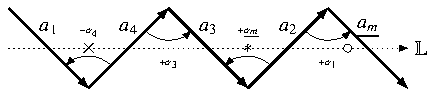
\includegraphics[width=0.64\textwidth]{figures/Fig_171_PDF280_Book268.pdf}
  \caption{带标记的弧、角与自旋翻转点（原书 p.268）}\label{fig:spin-morse-markers}
\end{figure}
\end{note}

\section{沿图粘合 Fukaya 范畴}\label{sec:gluing-categories}
\takeaway{沿带腿图粘合拓扑 Fukaya 范畴：带状图给出协变（余层）函子，管状图给出反变（层）函子，整体范畴是同伦（余）极限。圆柱的两个粘合例子分别把局部构件粘成 Kronecker 箭图与 $\mathbb P^1$ 的 $\mathbb Z_2$ 分次导出范畴。}
带标记曲面可以通过沿公共边粘合多边形构造；在 Fukaya 范畴层面也可以模拟这一过程。本节将讨论粘合 $A_\infty$ 范畴的几种方式。一般而言，粘合 $A_\infty$ 范畴或 dg 范畴需要用到高阶代数中的许多技巧，例如模型论\bookcite{239}及同伦（余）极限\bookcite{31,68}。这里仅在拓扑 Fukaya 范畴这一特殊情形中展示这些思想。一般框架的更多细节可参阅 Toen\bookcite{243,244}。

我们的目标是沿一种特定的一维空间粘合拓扑 Fukaya 范畴。此类空间由有限多个闭区间、半开区间和开区间组成，并将其中一些端点识别而得，称为带腿图 $\Gamma$。端点称为节点，区间称为边。根据区间的类型，边分为闭边、半开边和开边。半开边有时称为腿；开边不连接任何节点，有时称为孤立边。

图 $\Gamma$ 的每个具有有限多个连通分支的开子集，仍可视为带腿图。为排除具有无限多个连通分支的开集，我们将 $\mathrm{Open}(\Gamma)$ 定义为由所有有限多个连通分支的开集组成的范畴，态射为包含映射。若两个这样的开集 $\Upsilon_1,\Upsilon_2$ 的交为 $\Upsilon_{12}:=\Upsilon_1\cap\Upsilon_2$，则在 $\mathrm{Open}(\Gamma)$ 中有粘合图：
\begin{figure}[H]\centering
  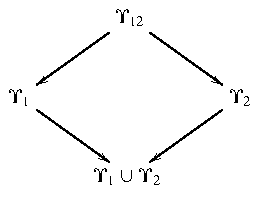
\includegraphics[width=0.35\textwidth]{figures/Fig_172_PDF281_Book269.pdf}
  \caption{开覆盖的粘合图式（原书 p.269）}\label{fig:open-cover-gluing-diagram}
\end{figure}
范畴论地说，$\Upsilon_1\cup\Upsilon_2$ 是图式 $\Upsilon_1\leftarrow\Upsilon_{12}\to\Upsilon_2$ 的余极限，因为任何补全该图式的方式都唯一地经由它分解。

\subsection*{沿带状图\index{daizhuangtu@带状图|hyperpage}粘合}
\begin{definition}{弧系的带状图}{ribbon-graph}
设 $A$ 是带标记曲面 $(S,M)$ 的生成弧系，并假设所有边界段都属于 $A$。带状图 $\Gamma_A$ 是一个带腿图：每个多边形中心对应一个节点；每条内部弧对应一条闭边；每条边界弧对应一条半开边。各边连接到弧所围多边形对应的节点。\footnote{之所以称为带状图，是因为它在 $(S,M)$ 中的自然嵌入允许我们把边加粗为带。}

对每个开集 $\Upsilon\in\mathrm{Open}(\Gamma_A)$，可以构造一个新的带标记曲面 $(S_\Upsilon,M_\Upsilon)$：把子图中各节点对应的多边形，沿 $\Upsilon$ 中闭边所对应的弧粘在一起。若 $\Upsilon$ 中含有孤立边，则为每条孤立边添加一个带两个标记点的圆盘。多边形的角就是 $S_\Upsilon$ 的标记点。
\end{definition}

\begin{theorem}{带状图上的协变范畴值函子}{ribbon-graph-cosheaf-functor}
存在一个协变函子，从范畴 $\mathrm{Open}(\Gamma_A)$ 出发，取值于以 $A_\infty$ 函子为态射的导出 $A_\infty$ 范畴所构成的范畴，并将每个 $\Upsilon$ 映到 $(S_\Upsilon,M_\Upsilon)$ 的拓扑 Fukaya 范畴：
\[
  R\colon\mathrm{Open}(\Gamma_A)\longrightarrow\mathrm{DCAT}_\infty,
  \qquad \Upsilon\longmapsto\mathrm{topFuk}^{\pm}(S_\Upsilon,M_\Upsilon).
\]
\end{theorem}
\begin{proof}[证明思路]
设 $\phi\colon\Upsilon_1\to\Upsilon_2$ 是 $\mathrm{Open}(\Gamma_A)$ 中的态射。对 $(S_{\Upsilon_i},M_{\Upsilon_i})$，取由各多边形边组成的弧系 $A_i$。态射 $\phi$ 诱导弧系之间的映射 $A_1\to A_2$，因为 $\Upsilon_1$ 中的每条边都落在 $\Upsilon_2$ 中唯一一条边上。这一映射未必是单射：$A_1$ 中两条弧可能映到 $A_2$ 中同一条弧。

每个非平凡角都唯一对应于一个多边形及两条入弧（对偶地，对应于一个节点及两条边），所以 $\phi$ 也诱导角之间的映射，从而得到 gentle 代数态射
\[
  F\colon\mathrm{Gtl}^{\pm}A_1\longrightarrow\mathrm{Gtl}^{\pm}A_2.
\]
这个态射保持 $A_\infty$ 结构：若某个角同时出现在两个曲面中，就表示相应多边形也同时出现在两者中。因此，在 $S_{\Upsilon_2}$ 中的任意多边形浸入也会出现在 $S_{\Upsilon_1}$ 中。转到导出范畴后得到严格的 $A_\infty$ 函子
\[
  R(\Upsilon_i):=D\mathrm{Gtl}^{\pm}A_i,
  \qquad R(\phi):=DF\colon R(\Upsilon_1)\longrightarrow R(\Upsilon_2).
\]
复合律由构造直接得到。\hfill$\square$
\end{proof}

函子 $R$ 很像一个预层，只是它由协变函子而非反变函子定义；换言之，它是一个余预层。甚至可以把 $R$ 称为 $A_\infty$ 范畴的余层。这表示，正如层的整体截面可以由局部截面沿交集相容地粘合而成，范畴 $R(\Upsilon_1\cup\Upsilon_2)$ 也是如下图式的一个普适构造：
\begin{figure}[H]\centering
  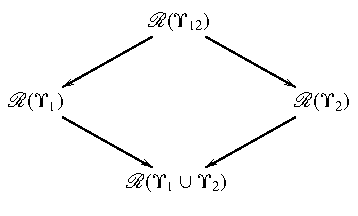
\includegraphics[width=0.45\textwidth]{figures/Fig_173_PDF283_Book271.pdf}
  \caption{范畴余层的粘合图式（原书 p.271）}\label{fig:categorical-cosheaf-diagram}
\end{figure}
数学上，$R(\Upsilon_1\cup\Upsilon_2)$ 是图式 $R(\Upsilon_1)\leftarrow R(\Upsilon_{12})\to R(\Upsilon_2)$ 的同伦余极限\index{tonglunyujixian@同伦余极限|hyperpage}。这是范畴中经典余极限的高阶版本，并且与拟同构和扭曲完备化相容。其精确定义超出本书范围；更多信息见 Haiden、Katzarkov 和 Kontsevich\bookcite{115}，Dyckerhoff 和 Kapranov\bookcite{65}，Sibilla、Treumann 和 Zaslow\bookcite{232}，Nadler\bookcite{189,188,191}，Pascaleff 和 Sibilla\bookcite{204}。

\begin{example}[由两个三角形粘合成圆柱]\label{ex:cylinder-ribbon-gluing}
可以把两个边界各有一个标记点的圆柱看成两个三角形沿边粘合而成：
\begin{figure}[H]\centering
  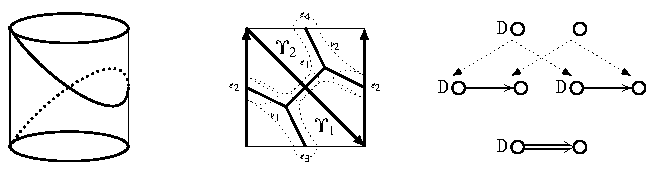
\includegraphics[width=0.86\textwidth]{figures/Fig_174_PDF283_Book271.pdf}
  \caption{圆柱的带状图及相应的箭图粘合（原书 p.271）}\label{fig:cylinder-ribbon-gluing}
\end{figure}
带状图有两个三价节点 $v_1,v_2$，由两条边 $e_1,e_2$ 相连；另有两条开边 $e_3,e_4$，分别连到 $v_1,v_2$。取开覆盖
\[
\begin{aligned}
  \Upsilon_1&=\{v_1\}\cup\operatorname{Int}(e_1)\cup\operatorname{Int}(e_2)\cup\operatorname{Int}(e_3),\\
  \Upsilon_2&=\{v_2\}\cup\operatorname{Int}(e_1)\cup\operatorname{Int}(e_2)\cup\operatorname{Int}(e_4),\\
  \Upsilon_{12}&=\operatorname{Int}(e_1)\cup\operatorname{Int}(e_2),
\end{aligned}
\]
则 Fukaya 范畴图式由两个线性箭图的导出范畴构成，二者都包含一个只有两个顶点、没有箭的箭图的导出范畴。其同伦余极限是沿这两个顶点粘合两个线性箭图所得的导出范畴，也就是 Kronecker 箭图的导出范畴。
\end{example}

\begin{note}\label{note:ribbon-graph-skeleton}
利用带状图粘合 Fukaya 范畴，是 Kontsevich 关于某些非紧辛流形的 wrapped Fukaya 范畴应由拉格朗日骨架\index{lagelangrigujia@拉格朗日骨架|hyperpage}构造这一思想的一维实现。拉格朗日骨架是辛流形的一个（可能奇异的）形变收缩核。它在骨架上给出一个范畴余层，相应的同伦余极限就是辛流形的 wrapped Fukaya 范畴。考察骨架的组合结构，便可把 wrapped Fukaya 范畴视为若干简单 $A_\infty$ 范畴的余极限。在这里，带状图就是拉格朗日骨架；简单部分对应于图节点的邻域（给出线性箭图 $L_n$ 的模范畴导出范畴 $D\mathrm{mod}^{\pm}L_n$）和边的邻域（给出 $\mathbb C$ 的导出范畴）。
\end{note}

\subsection*{沿管状图\index{guanzhuangtu@管状图|hyperpage}粘合}
\begin{definition}{切曲线与管状图}{tubular-graph}
设 $(S,M)$ 是带标记曲面。简单闭曲线是圆周 $S^1$ 到 $S$ 的一个嵌入，并且不与围绕某个内部标记点的小圆同伦。切集\index{qieji@切集|hyperpage} $C$ 是一组两两不相交且彼此不同伦的简单闭曲线。

由切集 $C$ 可构造一个带腿图，称为管状图 $\Gamma_C$。它的节点是删去这些简单闭曲线后所得的连通分支，边则对应简单闭曲线和内部标记点。对应简单闭曲线的边连接到该曲线围出的各连通分支所对应节点。其他边可视为半开边，因为它们只连接到包含相应标记点的节点。

与带状图情形相同，对每个开集 $\Upsilon\in\mathrm{Open}(\Gamma_C)$，都可构造一个新的带标记曲面：把 $\Upsilon$ 中节点对应的连通分支，沿其闭边所对应的闭曲线粘合；每条开边添加一个圆柱，并把未与内部标记点粘合的开端收缩。\footnote{在把标记点本身视为标记边界分支的形式体系中，最后一步并不需要，见第~\ref{note:marked-surface-conventions}~节的注记。}记所得曲面为 $(S_\Upsilon,M_\Upsilon)$。
\end{definition}

\begin{theorem}{管状图上的反变范畴值函子}{tubular-graph-sheaf-functor}
存在一个从范畴 $\mathrm{Open}(\Gamma_C)$ 到由导出 $A_\infty$ 范畴组成的范畴的反变函子；后者的态射为 $A_\infty$ 函子。该函子将每个 $\Upsilon$ 映到 $(S_\Upsilon,M_\Upsilon)$ 的拓扑 Fukaya 范畴：
\[
  T\colon\mathrm{Open}(\Gamma_C)^{\mathrm{op}}\longrightarrow\mathrm{DCAT}_\infty,
  \qquad \Upsilon\longmapsto\mathrm{topFuk}^{\pm}(S_\Upsilon,M_\Upsilon).
\]
\end{theorem}
\begin{proof}[证明思路]
取一个生成 $(S,M)$ 的弧系 $A$。给定 $\Upsilon\in\mathrm{Open}(\Gamma_C)$，每条弧 $a$ 都交替分解为位于 $(S_\Upsilon,M_\Upsilon)$ 内的弧段 $a_i$ 和不在其中的弧段 $b_i$。某些 $a_i$ 在 $(S_\Upsilon,M_\Upsilon)$ 中可能彼此同位变形，但它们合在一起仍能剖分 $S_\Upsilon$。将这组弧记为 $A_\Upsilon$，并令 $T(\Upsilon):=D\mathrm{Gtl}^{\pm}A_\Upsilon$。

若 $\phi\colon\Upsilon_1\to\Upsilon_2$ 是 $\mathrm{Open}(\Gamma_C)$ 中的态射，则 $A_{\Upsilon_2}$ 中每条弧 $a$ 都分解为若干子弧 $a_i$。映射
\[
  T\colon\mathrm{Gtl}^{\pm}A_{\Upsilon_2}\longrightarrow D\mathrm{Gtl}^{\pm}A_{\Upsilon_1},
  \qquad a\longmapsto\bigoplus_{a_i\subset a}a_i
\]
可以扩展为 $A_\infty$ 态射。若角 $\alpha$ 同时出现在 $S_{\Upsilon_2}$ 与 $S_{\Upsilon_1}$ 中，就令 $T(\alpha)=\alpha$，并把后者看成 $T(h(a))$ 与 $T(t(a))$ 的相应直和项之间的映射；若角 $\alpha$ 不出现在 $S_{\Upsilon_1}$ 中，则令 $T(\alpha)=0$。

考察 $A_{\Upsilon_1}$ 中弧之间的角，可见它们分成两类：一类也存在于 $S_{\Upsilon_2}$ 中，另一类是收缩闭曲线后新产生的角。后者可看成 $S_{\Upsilon_2}$ 中弧之间的弦。若 $S_{\Upsilon_2}\setminus S_{\Upsilon_1}$ 中的角序列 $a_0\leftarrow\cdots\leftarrow a_k$ 与一条弦 $\beta$ 围成浸入多边形，就令高阶分量 $T(\alpha_1,\ldots,\alpha_k)=\pm\beta$：
\begin{figure}[H]\centering
  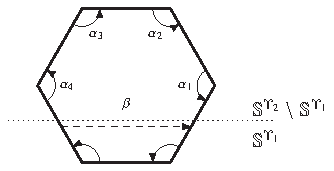
\includegraphics[width=0.44\textwidth]{figures/Fig_175_PDF285_Book273.pdf}
  \caption{收缩闭曲线后出现的高阶分量（原书 p.273）}\label{fig:tubular-gluing-higher-map}
\end{figure}
容易验证，这一赋值使 $T$ 成为 $A_\infty$ 态射。转到导出范畴后得到函子
\[
  T(\Upsilon_i):=D\mathrm{Gtl}^{\pm}A_i,
  \qquad T(\phi):=DT\colon T(\Upsilon_2)\longrightarrow T(\Upsilon_1).
\]
复合律由构造直接得到。\hfill$\square$
\end{proof}

\begin{note}\label{note:tubular-gluing-limit}
与带状图的情形相同，这个 $A_\infty$ 函子可以看成一个层，而范畴 $T(\Upsilon_1\cup\Upsilon_2)$ 可由图式
\[
T(\Upsilon_1)\longrightarrow T(\Upsilon_1\cap\Upsilon_2)\longleftarrow T(\Upsilon_2)
\]
通过同伦极限\index{tonglunjixian@同伦极限|hyperpage}构造。为使这一构造正常工作，必须对 Fukaya 范畴取 ind-完备化\footnote{例如，若 $\mathrm{topFuk}^{\pm}(\dot S)=D\mathrm{Mod}^{\pm}Q$，其 ind-完备化为 $D\mathrm{MOD}^{\pm}Q$。}。更多信息见 Pascaleff 和 Sibilla\bookcite{204}。请注意，由于采用了不同约定，他们把这种粘合称为沿闭子图粘合。
\end{note}

\begin{example}[沿闭曲线切开圆柱]\label{ex:cylinder-tubular-gluing}
仍考虑两个边界分支各有一个标记点的圆柱，并取一条把圆柱切成两半的简单闭曲线：
\begin{figure}[H]\centering
  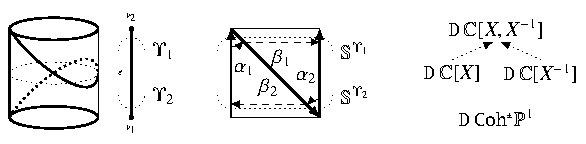
\includegraphics[width=0.94\textwidth]{figures/Fig_176_PDF286_Book274.pdf}
  \caption{圆柱切分、角及相应的代数图式（原书 p.274）}\label{fig:cylinder-tubular-gluing}
\end{figure}
管状图有两个一价节点 $v_1,v_2$，由一条边 $e$ 相连。每个节点对应一个边界上有一个标记点的穿孔圆盘，二者的交集是带有两个内部标记点的球面。取开覆盖
\[
  \Upsilon_1=v_1\cup\operatorname{Int}(e),\qquad
  \Upsilon_2=v_2\cup\operatorname{Int}(e),\qquad
  \Upsilon_{12}=\operatorname{Int}(e),
\]
则曲面 $S_{\Upsilon_1}$、$S_{\Upsilon_2}$ 都是边界上有一个标记点、内部有一个标记点的圆盘，而 $S_{\Upsilon_1\cap\Upsilon_2}$ 是开圆柱（或带两个标记点的球面）。

若取与例\ref{ex:cylinder-ribbon-gluing}相同的弧系，弧集 $\{a_1,a_2\}$ 在这三个曲面上都限制为两条弧。除原有角 $\alpha_1,\alpha_2\colon a_1\to a_2$ 外，交集曲面中还多出两个角 $\beta_1,\beta_2\colon a_2\to a_1$。角 $\beta_1$ 出现在 $S_{\Upsilon_2}$ 中，但不出现在 $S_{\Upsilon_1}$ 中；对 $\beta_2$ 则相反。相应的 gentle 代数由下列关系描述：
\[
\begin{aligned}
  \mathrm{Gtl}^{\pm}A_1&=\mathbb C\langle a_1,a_2,\alpha_1,\alpha_2,\beta_2\rangle
  /(\alpha_1\beta_2-1_{a_2},\,\beta_2\alpha_1-1_{a_1}),\\
  \mathrm{Gtl}^{\pm}A_2&=\mathbb C\langle a_1,a_2,\alpha_1,\alpha_2,\beta_1\rangle
  /(\alpha_2\beta_1-1_{a_2},\,\beta_1\alpha_2-1_{a_1}),\\
  \mathrm{Gtl}^{\pm}A_{12}&=\mathbb C\langle a_1,a_2,\alpha_1,\alpha_2,\beta_1,\beta_2\rangle
  /(\alpha_1\beta_2-1_{a_2},\,\beta_2\alpha_1-1_{a_1},\\
  &\hspace{39mm}\alpha_2\beta_1-1_{a_2},\,\beta_1\alpha_2-1_{a_1}).
\end{aligned}
\]

% [Tutor Note: 原书 p.274 把 $\mathrm{Gtl}^{\pm}A_2$ 的第二条关系印作 $\beta_1\alpha_1-1_{a_1}$，但 $\alpha_2$ 与 $\beta_1$ 才互为逆：$\alpha_2\beta_1=1_{a_2}$ 必须配 $\beta_1\alpha_2=1_{a_1}$。译文按后者写作 $\beta_1\alpha_2$；若沿用 $\beta_1\alpha_1$，该代数不会 Morita 等价于 $\mathbb C[\alpha_1\beta_1]$。]
由此得到相应的导出范畴粘合图式：
\begin{figure}[H]\centering
  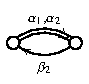
\includegraphics[width=0.9\textwidth]{figures/Fig_177_PDF286_Book274.pdf}
  \caption{两个区域中的第一组角关系（原书 p.274）}\label{fig:cylinder-tubular-algebra-one}
\end{figure}
\begin{figure}[H]\centering
  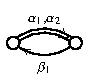
\includegraphics[width=0.9\textwidth]{figures/Fig_178_PDF286_Book274.pdf}
  \caption{两个区域中的第二组角关系（原书 p.274）}\label{fig:cylinder-tubular-algebra-two}
\end{figure}
\begin{figure}[H]\centering
  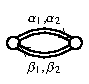
\includegraphics[width=0.9\textwidth]{figures/Fig_179_PDF286_Book274.pdf}
  \caption{交集曲面上的两组角关系（原书 p.274）}\label{fig:cylinder-tubular-algebra-intersection}
\end{figure}
因此，$\mathrm{Gtl}^{\pm}A_1$ 与 $\mathbb C[\alpha_2\beta_2]=\mathbb C[X]$ Morita 等价，$\mathrm{Gtl}^{\pm}A_2$ 与 $\mathbb C[\alpha_1\beta_1]=\mathbb C[Y]$ Morita 等价。最后，在 $\mathrm{Gtl}^{\pm}A_{12}$ 中，$\alpha_1\beta_1$ 与 $\beta_2\alpha_2$ 互为逆元，所以该代数与 $\mathbb C[X,Y]/(XY-1)$ Morita 等价。

这说明我们正在把 $\mathbb C[X]$ 与 $\mathbb C[X^{-1}]$ 的导出范畴沿 $\mathbb C[X,X^{-1}]$ 的导出范畴粘合。所得同伦极限是两条仿射直线沿 $\mathbb C^*$ 粘合后的导出范畴，换言之，就是 $\mathbb P^1$ 的 $\mathbb Z_2$ 分次导出范畴。
\end{example}

\section{粘合与镜像对称}\label{sec:gluing-mirror-symmetry}
\takeaway{裤子曲面 $(S^2,\{0,1,\infty\})$ 的拓扑 Fukaya 范畴等价于矩阵分解范畴 $\mathrm{MF}^{\pm}(\mathbb C^3,XYZ)$；用矩阵分解的 Čech 型粘合把裤子拼成高亏格曲面，得到非仿射 Landau--Ginzburg 模型，两侧图式的同伦极限互相对应。}
现在用上一节的粘合方法研究穿孔黎曼曲面的镜像对称。基本思路是先构造一个镜像对称的基本构件，再把多个这样的构件粘合起来。基本构件是裤子曲面\index{kuziqumian@裤子曲面|hyperpage}，也就是有三个标记点的球面\index{daisangebiaojidiandeqiumian@带三个标记点的球面|hyperpage} $(S^2,\{0,1,\infty\})$。其镜像对称由 Abouzaid、Auroux、Efimov、Katzarkov 和 Orlov\bookcite{1}建立。

\begin{theorem}{裤子曲面的镜像对称}{pants-mirror-equivalence}
裤子曲面的拓扑 Fukaya 范畴与 Landau--Ginzburg 模型 $(\mathbb C^3,XYZ)$ 的矩阵分解范畴导出等价：
\[
  \mathrm{topFuk}^{\pm}(S^2,\{0,1,\infty\})
  \cong_\infty \mathrm{MF}^{\pm}(\mathbb C^3,XYZ).
\]
\end{theorem}
\begin{proof}[证明思路]
把球面剖分成两个三角形，得到由三条弧 $\{x,y,z\}$ 组成的弧系。下图给出相应的曲面、三角剖分和箭图：
\begin{figure}[H]\centering
  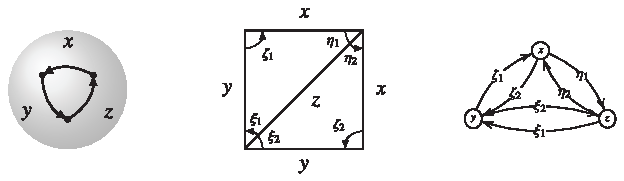
\includegraphics[width=0.91\textwidth]{figures/Fig_180_PDF287_Book275.pdf}
  \caption{裤子曲面的弧系、三角剖分及其箭图（原书 p.275）}\label{fig:pants-arcs-quiver}
\end{figure}
所有箭的次数都是 $1$，例如
\[
\begin{aligned}
  \mu(\zeta_1,\xi_1,\eta_1)=\mu(\eta_2,\xi_2,\zeta_2)&=1_x,\\
  \mu(\xi_1,\eta_1,\zeta_1)=\mu(\zeta_2,\eta_2,\xi_2)&=1_y,\\
  \mu(\eta_1,\zeta_1,\xi_1)=\mu(\xi_2,\zeta_2,\eta_2)&=1_z.
\end{aligned}
\]
$B$ 侧有三个显然的矩阵分解。令 $R=\mathbb C[X,Y,Z]$，则
\[
  M_X=\left(R^{\oplus2},\begin{pmatrix}0&X\\YZ&0\end{pmatrix}\right),\quad
  M_Y=\left(R^{\oplus2},\begin{pmatrix}0&Y\\XZ&0\end{pmatrix}\right),\quad
  M_Z=\left(R^{\oplus2},\begin{pmatrix}0&Z\\XY&0\end{pmatrix}\right).
\]
从 $M_Z$ 到 $M_Y$ 的 Hom 空间是 $\mathrm{Mat}_{2\times2}(R)$，其微分为
\[
  d\begin{pmatrix}a&b\\c&d\end{pmatrix}
  =\begin{pmatrix}0&Y\\XZ&0\end{pmatrix}\begin{pmatrix}a&b\\c&d\end{pmatrix}
   -\begin{pmatrix}a&-b\\-c&d\end{pmatrix}\begin{pmatrix}0&Z\\XY&0\end{pmatrix}
  =\begin{pmatrix}Yc+bXY&Yd-aZ\\XZa-dXY&XZb+cZ\end{pmatrix}.
\]
该空间的上同调为 $\mathbb C[X]\xi_1$，其中
\[
  \xi_1=\begin{pmatrix}0&-1\\X&0\end{pmatrix}.
\]
类似计算给出下表（表中非对角项表示由相应矩阵生成的多项式模）：
{\small
\[
\begin{array}{c|ccc}
  &M_X&M_Y&M_Z\\\hline
M_X&\mathbb C[Y]1+\mathbb C[Z]1
&\mathbb C[Z]\!\begin{pmatrix}0&-1\\Z&0\end{pmatrix}
&\mathbb C[Y]\!\begin{pmatrix}0&-1\\Y&0\end{pmatrix}\\[5pt]
M_Y&\mathbb C[Z]\!\begin{pmatrix}0&-1\\Z&0\end{pmatrix}
&\mathbb C[Z]1+\mathbb C[X]1
&\mathbb C[X]\!\begin{pmatrix}0&-1\\X&0\end{pmatrix}\\[5pt]
M_Z&\mathbb C[Y]\!\begin{pmatrix}0&-1\\Y&0\end{pmatrix}
&\mathbb C[X]\!\begin{pmatrix}0&-1\\X&0\end{pmatrix}
&\mathbb C[X]1+\mathbb C[Y]1
\end{array}
\]
}
根据矩阵中出现的变量，把六个次数为 $1$ 的生成元记为 $\xi_1,\xi_2,\ldots,\zeta_1,\zeta_2$。只有希腊字母相同的乘积非零。例如
\[
  \zeta_1\eta_1=
  \begin{pmatrix}0&-1\\Z&0\end{pmatrix}
  \begin{pmatrix}0&-1\\Y&0\end{pmatrix}
  =\begin{pmatrix}-Y&0\\0&-Z\end{pmatrix}
  =d\begin{pmatrix}0&0\\1&0\end{pmatrix}.
\]
所以这六个次数为 $1$ 的态射的行为恰好与上述弧系中的角相同。令 $M=M_X\oplus M_Y\oplus M_Z$，便有
\[
  \mathrm{MF}^{\pm}(M,M)\cong\mathrm{Gtl}^{\pm}A.
\]
这个代数同构可提升为 $A_\infty$ 同构。例如，为验证 $\mu(\zeta_1,\xi_1,\eta_1)=1_{M_X}$，取分解使
\[
  \begin{pmatrix}0&0\\0&1\end{pmatrix}\in R,
  \qquad
  \begin{pmatrix}-X&0\\0&-Y\end{pmatrix}
  =d\begin{pmatrix}0&0\\-1&0\end{pmatrix}\in I.
\]
于是
\[
\begin{aligned}
  \mu(\zeta_1,\xi_1,\eta_1)
  &=\pi\begin{pmatrix}0&-1\\Z&0\end{pmatrix}
    h\!\left(\begin{pmatrix}0&-1\\Y&0\end{pmatrix}
             \begin{pmatrix}0&-1\\X&0\end{pmatrix}\right)
   +\pi h\!\left(\begin{pmatrix}0&-1\\Z&0\end{pmatrix}
             \begin{pmatrix}0&-1\\Y&0\end{pmatrix}\right)
             \begin{pmatrix}0&-1\\X&0\end{pmatrix}\\
  &=\pi\begin{pmatrix}0&-1\\Z&0\end{pmatrix}
    h\begin{pmatrix}-X&0\\0&-Y\end{pmatrix}
   +\pi h\begin{pmatrix}-Y&0\\0&-Z\end{pmatrix}
             \begin{pmatrix}0&-1\\X&0\end{pmatrix}\\
  &=\pi\begin{pmatrix}0&-1\\Z&0\end{pmatrix}
    \begin{pmatrix}0&0\\-1&0\end{pmatrix}
   +\pi\begin{pmatrix}0&0\\-1&0\end{pmatrix}
             \begin{pmatrix}0&-1\\X&0\end{pmatrix}\\
  &=\pi\begin{pmatrix}1&0\\0&0\end{pmatrix}
   +\pi\begin{pmatrix}0&0\\0&1\end{pmatrix}=1_{M_X}.
\end{aligned}
\]
% [Tutor Note: 原书 p.276 这一推导的末行印作 $=-\,\mathbb{1}$，与所要证的 $\mu(\zeta_1,\xi_1,\eta_1)=1_{M_X}$ 矛盾；译文取 $1_{M_X}$。若按原书取 $-1$，则须同步改变 $\mu(\zeta_1,\xi_1,\eta_1)=1_x$ 的符号约定，属原书笔误。]
与其逐一检查所有非零高阶乘积，不如证明 $\mu(\zeta_1,\xi_1,\eta_1)$ 和 $\mu(\eta_2,\xi_2,\zeta_2)$ 的取值唯一确定代数 $\mathrm{Gtl}^{\pm}A$ 上的 $A_\infty$ 结构（至 $A_\infty$ 同构）。这可以用 $A_\infty$ 代数的变形理论和 Hochschild 上同调证明；第\ref{ch:deformation}章，尤其是定理\ref{thm:ainfty-deformation-classification}，将更详细地说明这一点。

证明的最后一步是说明这三个矩阵分解生成 $\mathrm{MF}^{\pm}(\mathbb C^3,XYZ)$。由定理\ref{thm:buchweitz-singularity-category}，矩阵分解范畴等价于 $X=W^{-1}(0)$ 的奇点范畴；$X$ 由三个坐标平面组成。在这一对应下，$M_X[1]$ 对应于 $R/(X)$，即 $YZ$ 平面的结构层。由于 $YZ$ 平面光滑，其结构层生成该平面的导出范畴。在 $D^b\mathrm{Coh}X$ 中，$R/(X)$ 生成所有支撑在 $YZ$ 平面上的层。因此，$D^b\mathrm{Coh}X$ 由 $R/(X),R/(Y),R/(Z)$ 生成，奇点范畴也由这些对象生成。证明的更多细节见\bookcite{1,155}。\hfill$\square$
\end{proof}

\begin{note}\label{note:pants-singularity-mirror}
矩阵分解范畴描述了 $\mathbb C^3$ 中 $XYZ=0$ 的奇点集。这个奇点集由三条在原点相接的仿射直线组成。对奇点集上的每一点，都可以为该点的点层构造局部自由分解，并考察其二周期尾部，从而得到矩阵分解。对 $p=(0,0,z)$，所得矩阵分解为
\[
  M_p=\left(\begin{array}{cccc}
  0&X&0&0\\YZ&0&0&0\\Z-z&0&0&X\\0&z-Z&YZ&0
  \end{array}\right)=\operatorname{Cone}(\zeta_1\ \ \zeta_2-z).
\]
它对应于裤子曲面上绕某个标记点的圆周 $L_p$，并带有绕行变换为 $z$ 的局部系统。

对原点，得到矩阵分解 $R\otimes\Lambda_3$，其微分为
\[
  d\phi:=\iota_X\phi+\iota_Y\phi+\iota_Z\phi
  +(YZ\,dX+XZ\,dY+XY\,dZ)\wedge\phi.
\]
该矩阵分解与下列对象拟同构：
\[
  M_0=\operatorname{Cone}\!\left(
  M_x\oplus M_y\oplus M_z\xrightarrow{\ \xi_1\pm\cdots\pm\zeta_2\ }
  M_x\oplus M_y\oplus M_z\right).
\]
它对应于一条环绕裤子曲面“裆部”的曲线 $L_0$，其局部系统的绕行变换为 $\lambda=-1$。\footnote{文献\bookcite{71,220}中通过非平凡自旋结构实现这一局部系统。}

最后，三个矩阵分解 $M_X,M_Y,M_Z$ 分别对应于支撑在三条仿射直线中两条上的对象。注意，$p=(0,0,z)$ 处的 $M_p$ 可以看成 $M_X$ 或 $M_Y$ 上的锥，却不能看成 $M_Z$ 上的锥。因此，$p$ 属于 $M_X,M_Y$ 的支撑，而不属于 $M_Z$ 的支撑。从 $A$ 侧看这一点也很清楚：$L_p$ 与弧 $x,y$ 相交，但不与 $z$ 相交。
\begin{figure}[H]\centering
  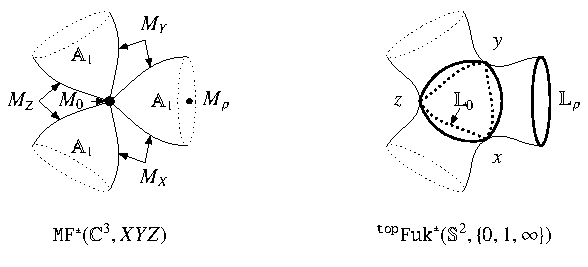
\includegraphics[width=0.93\textwidth]{figures/Fig_181_PDF290_Book278.pdf}
  \caption{裤子曲面上的矩阵分解与曲线对象（原书 p.278）}\label{fig:pants-singularity-objects}
\end{figure}
\end{note}

这个镜像对应也与粘合相容。下面说明如何把不同的裤子曲面粘在一起，从而为亏格较高、标记点较多的曲线构造非仿射 Landau--Ginzburg 模型。

\begin{example}[粘合裤子曲面得到四标记球面的镜像]\label{ex:gluing-pants-landau-ginzburg}
取 $U_1,U_2\cong\mathbb C^3$，其中 $U_i=V(R_i)$，$R_i=\mathbb C[X_i,Y_i,Z_i]$。要把这两个仿射空间粘起来，可取一个过渡映射，使 $X_1Y_1Z_1$ 与 $X_2Y_2Z_2$ 对应，并把其中一个坐标取逆。例如
\[
  X_2=X_1Z_1,\qquad Y_2=Y_1Z_1,\qquad Z_2=Z_1^{-1}.
\]
交集 $U_{12}$ 是环
\[
  R_{12}=\mathbb C[X_1,Y_1,Z_1^{\pm1}]
  =\mathbb C[X_2,Y_2,Z_2^{\pm1}]
\]
所对应的簇，且该环含有函数 $\ell=X_1Y_1Z_1=X_2Y_2Z_2$。

嵌入 $U_{12}\hookrightarrow U_i$ 诱导限制函子
\[
  \mathrm{MF}^{\pm}(R_i,\ell)\longrightarrow\mathrm{MF}^{\pm}(R_{12},\ell),
  \qquad (M,d)\longmapsto(M\otimes_{R_i}R_{12},d\otimes_{R_i}1).
\]
若把矩阵分解 $M_X,M_Y,M_Z$ 限制到交集，会发生什么？把 $Z$ 取逆后，态射 $\zeta_1,\zeta_2$ 变成可逆态射，矩阵分解 $M_Z$ 成为零对象，因为
\[
  1_{M_Z}=
  \begin{pmatrix}0&Z\\XY&0\end{pmatrix}
  \begin{pmatrix}0&0\\Z^{-1}&0\end{pmatrix}
  +\begin{pmatrix}0&0\\Z^{-1}&0\end{pmatrix}
  \begin{pmatrix}0&Z\\XY&0\end{pmatrix}
  =d\begin{pmatrix}0&0\\Z^{-1}&0\end{pmatrix}.
\]
因此，在 $\mathrm{MF}^{\pm}(R_{12},\ell)$ 中，$M_X\cong M_Y[1]$ 且 $M_Z=0$。此外，$M_X$ 的自同态环为 $\mathbb C[Z,Z^{-1}]1_{M_X}$，所以
\[
  \mathrm{MF}^{\pm}(\mathbb C[X,Y,Z,Z^{-1}],XYZ)
  \cong_\infty D\mathbb C[Z,Z^{-1}],
\]
它也就是两个标记点的球面的 Fukaya 范畴。若沿 $U_{12}$ 把 $U_1$ 与 $U_2$ 粘起来，就得到一个簇 $X$，其全局函数为 $\ell=X_1Y_1Z_1=X_2Y_2Z_2$；这就是一个非仿射 Landau--Ginzburg 模型。

范畴 $\mathrm{MF}^{\pm}(X,\ell)$ 的对象是二元组 $(P,d)$，其中 $P$ 是 $\mathbb Z_2$ 分次局部自由层，且 $d\in\mathrm{Hom}(P,P)$ 满足 $d^2=\ell$。局部自由层由三元组 $(R_1^n,R_2^n,U)$ 确定，其中 $U\in\mathrm{Mat}_{n\times n}(R_{12})$ 可逆。微分由一对映射 $d_1,d_2$ 给出，满足
\[
  (d_1^2,d_2^2)=(X_1Y_1Z_1,X_2Y_2Z_2),\qquad d_1=Ud_2U^{-1}
\]
（后一等式在 $R_{12}$ 上成立）。由此可以构造四个矩阵分解：
{\scriptsize
\[
\begin{array}{c|c|c|c}
 &d_1&d_2&U\\\hline
M_{Z_1}&\begin{pmatrix}0&Z_1\\X_1Y_1&0\end{pmatrix}
&\begin{pmatrix}0&1\\X_2Y_2Z_2&0\end{pmatrix}
&\begin{pmatrix}Z_1&0\\0&1\end{pmatrix}\\[7pt]
M_{Z_2}&\begin{pmatrix}0&1\\X_1Y_1Z_1&0\end{pmatrix}
&\begin{pmatrix}0&Z_2\\X_2Y_2&0\end{pmatrix}
&\begin{pmatrix}Z_1&0\\0&1\end{pmatrix}\\[7pt]
M_X&\begin{pmatrix}0&X_1\\Y_1Z_1&0\end{pmatrix}
&\begin{pmatrix}0&X_2\\Y_2Z_2&0\end{pmatrix}
&\begin{pmatrix}Z_1^{-1}&0\\0&1\end{pmatrix}\\[7pt]
M_Y&\begin{pmatrix}0&Y_1\\X_1Z_1&0\end{pmatrix}
&\begin{pmatrix}0&Y_2\\X_2Z_2&0\end{pmatrix}
&\begin{pmatrix}Z_1^{-1}&0\\0&1\end{pmatrix}
\end{array}
\]
}
两个对象 $(P,d_P)$ 与 $(Q,d_Q)$ 之间的态射空间，是 $\mathrm{Hom}(P,Q)$ 的 Čech 复形，其微分为 $d_C+d_{\mathrm{MF}}$：
\[
\begin{gathered}
  \check C=(\mathrm{Mat}_{n\times m}(R_1)\oplus
  \mathrm{Mat}_{n\times m}(R_2)\oplus\mathrm{Mat}_{n\times m}(R_{12})),\\
  d(\phi_1,\phi_2,\phi_{12})=\bigl(
  d_{Q_1}\phi_1-(-1)^{|\phi|}\phi_1d_{P_1},\;
  d_{Q_2}\phi_2-(-1)^{|\phi|}\phi_2d_{P_2},\\[-2pt]
  d_{Q_1}\phi_{12}-(-1)^{|\phi|}\phi_{12}d_{P_1}
  +\phi_1-U_Q\phi_2U_P^{-1}\bigr).
\end{gathered}
\]
计算 $\mathrm{MF}^{\pm}(M,M)$ 的极小模型，其中 $M=M_{Z_1}\oplus M_{Z_2}\oplus M_X\oplus M_Y$，得到如下箭图：
\begin{figure}[H]\centering
  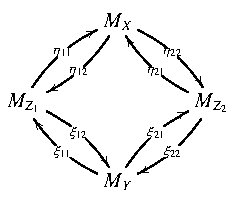
\includegraphics[width=0.56\textwidth]{figures/Fig_182_PDF291_Book279.pdf}
  \caption{粘合矩阵分解的极小模型箭图（原书 p.279）}\label{fig:glued-mf-minimal-quiver}
\end{figure}
所有 $\xi_{ij}$、$\eta_{ij}$ 都具有形如 $(\phi_1,\phi_2,0)$ 的形式，其中 $\phi_1\otimes_{R_1}R_{12}=\phi_2\otimes_{R_2}R_{12}$。例如
\[
  \xi_{11}=\left(\left(
  \begin{pmatrix}0&-1\\X_1&0\end{pmatrix},
  \begin{pmatrix}0&-1\\X_2Z_2&0\end{pmatrix}\right),0\right).
\]
进一步确定 $A_\infty$ 结构可得
\[
  \mu(\xi_{12},\eta_{12},\xi_{22},\eta_{22})=1_{M_X},
\]
并且 $\mathrm{MF}^{\pm}(M,M)$ 与四标记点球面上正方形四边的自同态环之间存在 $A_\infty$ 同构。对应关系图示如下：
\begin{figure}[H]\centering
  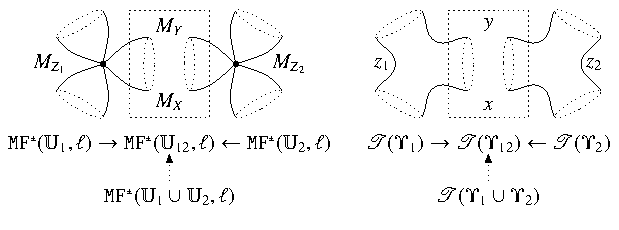
\includegraphics[width=0.93\textwidth]{figures/Fig_183_PDF292_Book280.pdf}
  \caption{Landau--Ginzburg 模型粘合与曲面范畴粘合的对应（原书 p.280）}\label{fig:glued-mf-surface-diagrams}
\end{figure}
两侧的图式都是由等价图式取同伦极限得到，因此
\[
  \mathrm{MF}^{\pm}(X,\ell)\cong_\infty
  \mathrm{topFuk}^{\pm}(S^2,\{0,1,\infty,p\}).
\]

这一思路可推广到亏格更高、标记点更多的曲面。取 $\mathbb Z^2$ 中一个凸格多边形，其内部有 $g$ 个格点、边界上有 $n$ 个格点，并把它放在 $\mathbb Z^3$ 中高度 $z=1$ 的平面上。令 $P$ 为多边形中的格点集，对每个 $p\in P$，记其坐标为 $(a_p,b_p,1)$。

选取一个三角剖分 $T$，把多边形分成基本三角形。基本三角形是 $v=\{r,s,t\}\subset P$，除顶点外不含其他格点；等价地，$r,s,t$ 构成 $\mathbb Z^3$ 的一组基。对每个三角形定义子环
\[
  R_v=\mathbb C[X^iY^jZ^k\mid a_pi+b_pj+k\ge0,\ p\in v],
  \qquad U_v=V(R_v).
\]
因为 $r,s,t$ 构成 $\mathbb Z^3$ 的一组基，$R_v$ 同构于三元多项式环，故 $U_v\cong\mathbb C^3$。$R_v$ 的生成元是单项式 $X^iY^jZ^k$，其中 $(i,j,k)$ 是 $r,s,t$ 的对偶基。把这些单项式记作 $U_v,V_v,W_v$。由于 $r,s,t$ 都位于平面 $z=1$，有
\[
  Z=U_vV_vW_v.
\]

对每条边 $e=\{r,s\}$，定义
\[
  R_e=\mathbb C[X^iY^jZ^k\mid a_pi+b_pj+k\ge0,\ p\in e].
\]
它同构于 $\mathbb C[U_v,V_v,W_v,W_v^{-1}]$，因为此处少了第三个不等式条件。因此 $U_e=V(R_e)\cong\mathbb C^2\times\mathbb C^*$。若 $e$ 是三角形 $v$ 的一条边，则 $R_v\subset R_e$，对偶地 $U_e\subset U_v$。沿公共边识别各个 $U_e$ 并粘合所有 $U_v$，得到一个三维光滑环簇 $Y_T$。所有这些环都是 $\mathbb C[X^{\pm1},Y^{\pm1},Z^{\pm1}]$ 的子环，并且都含有 $\ell=Z$。因此 $\ell$ 是 $Y_T$ 上的全局函数，我们得到 Landau--Ginzburg 模型 $(Y_T,\ell)$。

现在考察三角剖分的对偶图 $\Gamma_T$。每个三角形对应一个节点，每条剖分边对应一条对偶边；若原边位于多边形边界上，则对应的对偶边是半开边。每个节点 $v$ 带有 Landau--Ginzburg 模型 $(U_v,\ell)$，每条边带有模型 $(U_e,\ell)$。若边 $e$ 与节点 $v$ 相连，则有嵌入 $U_e\hookrightarrow U_v$。
\begin{figure}[H]\centering
  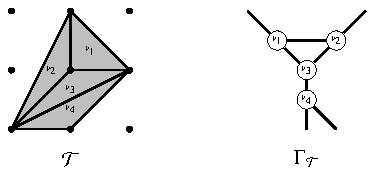
\includegraphics[width=0.79\textwidth]{figures/Fig_184_PDF293_Book281.pdf}
  \caption{三角剖分及其对偶图（原书 p.281）}\label{fig:triangulation-dual-graph}
\end{figure}
对每个节点 $v$ 和边 $e$，有两个矩阵分解范畴及一个限制函子：
\[
  \mathcal M(U_v):=\mathrm{MF}^{\pm}(U_v,\ell)
  \longrightarrow
  \mathcal M(U_e):=\mathrm{MF}^{\pm}(U_e,\ell).
\]
由此得到一个 $A_\infty$ 范畴图式；$(Y_T,\ell)$ 的矩阵分解范畴可以解释为该图式的同伦极限。

$A$ 侧则沿对偶图 $\Gamma_T$ 构造管状邻域 $\Sigma_T$，得到一个带穿孔曲面，其亏格等于图中的圈数，穿孔数等于管状图的腿数。用多边形来表述，亏格等于多边形内部格点数，腿数等于边界格点数。可用节点周围的开星形邻域 $\Upsilon_v$ 和边的开邻域 $\Upsilon_e$ 覆盖该图。应用函子 $T$ 后，也得到 Fukaya 范畴图式，其同伦极限为 $\mathrm{topFuk}^{\pm}(\Sigma_T)$。下图展示了两个对应的图式：
\begin{figure}[H]\centering
  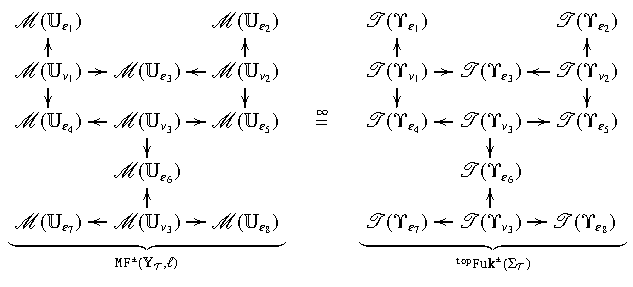
\includegraphics[width=0.98\textwidth]{figures/Fig_185_PDF293_Book281.pdf}
  \caption{矩阵分解范畴与拓扑 Fukaya 范畴图式的对应（原书 p.281）}\label{fig:triangulation-category-diagrams}
\end{figure}
核心想法是：这两个图式 $A_\infty$ 等价，因此它们的极限也等价。
\end{example}

\begin{theorem}{Sibilla--Pascaleff--Lee 定理}{polygon-gluing-mirror-equivalence}
设 $T$ 是一个凸格多边形的三角剖分，多边形内部有 $g$ 个格点、边界有 $n$ 个格点，则
\[
  \mathrm{MF}^{\pm}(Y_T,\ell)\cong_\infty\mathrm{topFuk}^{\pm}(\Sigma_T),
\]
其中 $\Sigma_T$ 是亏格为 $g$、有 $n$ 个标记点的闭带标记曲面。
\end{theorem}
\begin{proof}[证明思路]
为使上述构想成立，必须转到适当完备化后的范畴。先在完备化的设定中作粘合，再把所得等价限制到紧对象子范畴，就得到未完备化版本之间的等价。更多细节见 Pascaleff 和 Sibilla\bookcite{204}。Lee 的另一种方法是分别识别两侧的生成元，见\bookcite{155}。\hfill$\square$
\end{proof}

\section{覆盖}\label{sec:covers}
\takeaway{覆盖 $\pi$ 拉回弧系给出严格 $A_\infty$ 函子，而群作用与叉积 $A\star G$ 给出覆盖曲面的 gentle 代数；据此为商栈 $[\mathbb C^3/G]$ 构造带栈镜像，其标记点数由特征标 $\lambda_X,\lambda_Y,\lambda_Z$ 的稳定子决定。}
\begin{definition}{带标记曲面间的覆盖映射}{marked-surface-cover}
设 $(S_1,M_1)$、$(S_2,M_2)$ 是带标记曲面。映射 $\pi\colon S_1\to S_2$ 称为覆盖映射\index{daibiaojiqumianjiandefugaiyingshe@带标记曲面间的覆盖映射|hyperpage}，若它是一个分支覆盖，满足 $\pi(M_1)=M_2$，且所有分支点都位于 $M_2$。覆盖次数定义为 $p\in S_2\setminus M_2$ 的原像点数 $|\pi^{-1}(p)|$。
\end{definition}

若 $A_2$ 是剖分 $(S_2,M_2)$ 的弧系，则沿 $\pi$ 拉回 $A_2$，得到剖分 $(S_1,M_1)$ 的弧系 $A_1$。$A_1$ 中任意两条弧之间的角态射都会映到 $S_2$ 中的一个角态射。因此，$\pi$ 诱导 gentle 范畴之间的严格 $A_\infty$ 函子
\[
  F_\pi\colon\mathrm{Gtl}^{\pm}A_1\longrightarrow\mathrm{Gtl}^{\pm}A_2,
  \qquad a\longmapsto\pi(a),\quad\alpha\longmapsto\pi(\alpha),
\]
并可扩张为导出范畴或相应拓扑 Fukaya 范畴之间的函子。类似地，覆盖 $\pi$ 的自同构群
\[
  G=\{\phi\colon S_1\to S_1\mid \pi\phi=\pi\}
\]
作用在弧系 $A_1$ 上，由此也得到严格 $A_\infty$ 函子对 $\mathrm{Gtl}^{\pm}A_1$ 的作用。现在反过来考虑这个构造。

\begin{definition}{群作用的 $A_\infty$ 代数叉积}{ainfty-smash-product}
设 $A$ 是一个 $A_\infty$ 代数，有限群 $G$ 通过严格 $A_\infty$ 同构作用于 $A$。叉积\index{chaji@叉积|hyperpage}代数定义为 $A\star G:=A\otimes\mathbb CG$，其 $A_\infty$ 乘积为
\[
  \mu(a_1\otimes g_1,\ldots,a_k\otimes g_k)
  =\mu(a_1,g_1\cdot a_2,\ldots,g_1\cdots g_{k-1}\cdot a_k)
  \otimes g_1\cdots g_k.
\]
容易验证，这些乘积满足 $A_\infty$ 公理。
\end{definition}

设 $A=\mathbb C Q/I$ 是由带标记曲面 $(S,M)$ 上弧系 $A$ 所给出的 gentle $A_\infty$ 代数，并且阿贝尔群 $G$ 的作用固定各顶点、只对每个角乘以一个标量。具体说，对每个 $\alpha\in Q_1$，存在一个特征标 $\lambda_\alpha\in\widehat G=\mathrm{Grp}(G,\mathbb C^*)$，使得 $g\cdot\alpha=\lambda_\alpha(g)\alpha$；若 $\alpha_1,\ldots,\alpha_k$ 是某个多边形的各角，则 $\lambda_{\alpha_1}\cdots\lambda_{\alpha_k}=1$。

\begin{theorem}{覆盖与 gentle 代数叉积}{gentle-cover-smash-product}
在上述设定下，
\[
  A\star G\cong\mathrm{Gtl}^{\pm}\widetilde A,
\]
其中 $\widetilde A$ 是 $A$ 沿覆盖 $\pi\colon\widetilde S\to S$ 拉回所得的弧系。
\end{theorem}
\begin{proof}[证明思路]
对每个 $\lambda\in\widehat G$ 及 $a\in Q_0$，定义
\[
  e_\lambda:=\frac1{|G|}\sum_{g\in G}\lambda(g)g\in\mathbb CG,
  \qquad a_\lambda:=a\otimes e_\lambda\in A\star G.
\]
$e_\lambda$ 构成 $\mathbb CG$ 的一组正交幂等基，而 $a_\lambda$ 构成 $A\star G$ 的一组完备正交幂等元。把 $a_\lambda$ 作为新箭图 $\widetilde Q$ 的顶点。若 $\alpha\in Q_1$ 是一条从 $b=t(\alpha)$ 到 $a=h(\alpha)$ 的角，则
\[
\begin{aligned}
  \alpha\otimes1
  &=\left(\sum_{\kappa\in\widehat G}a\otimes e_\kappa\right)
    (\alpha\otimes1)
    \left(\sum_{\lambda\in\widehat G}b\otimes e_\lambda\right)\\
  &=\sum_{\kappa,\lambda\in\widehat G}
    (a\otimes e_\kappa)(\alpha\otimes e_{\kappa\lambda_\alpha})
    (b\otimes e_\lambda)\\
  &=\sum_{\kappa\in\widehat G}
    (a\otimes e_\kappa)(\alpha\otimes1)(b\otimes e_{\kappa\lambda_\alpha})\\
  &=\sum_{\kappa\in\widehat G}a_\kappa(\alpha\otimes1)b_{\kappa\lambda_\alpha}.
\end{aligned}
\]
因此 $\alpha\otimes1$ 分解为 $\widetilde Q$ 中 $|G|$ 条新箭 $\alpha_\kappa$，其头尾满足
\[
  h(\alpha_\kappa)=h(\alpha)_\kappa,
  \qquad t(\alpha_\kappa)=t(\alpha)_{\kappa\lambda_\alpha}.
\]
若 $\alpha_1,\ldots,\alpha_k$ 是 $S$ 中某个多边形的各角，则对每个 $\kappa\in\widehat G$，用下列各角作为边界可构造一个新的多边形：
\[
  (\alpha_1)_\kappa,\quad
  (\alpha_2)_{\kappa\lambda_{\alpha_1}},\quad\ldots,\quad
  (\alpha_k)_{\kappa\lambda_{\alpha_1}\cdots\lambda_{\alpha_{k-1}}}.
\]
把这些多边形粘合起来，得到新曲面 $\widetilde S$ 及其弧系 $\widetilde A=\widetilde Q_0$，相应 gentle $A_\infty$ 代数同构于 $A\star G$。\hfill$\square$
\end{proof}

\begin{example}[三标记球面的三重覆盖]\label{ex:threefold-pants-cover}
取一个有三个标记点的球面，并构造一个以环面为覆盖空间、以这三个标记点为分支点的三重覆盖。球面上的三角形给出弧系 $A_2=\{x,y,z\}$；沿覆盖拉回后得到弧系
\[
  A_1=\{x_1,x_2,x_3,\ldots,z_1,z_2,z_3\}.
\]
可以把它画成平面上的周期弧系，其基本区域由六个三角形组成。覆盖自同构群为 $\mathbb Z_3$，并循环置换各弧的下标。
\begin{figure}[H]\centering
  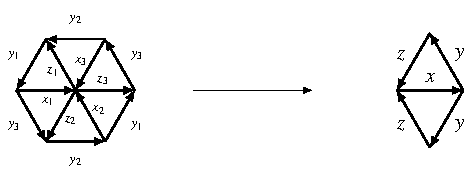
\includegraphics[width=0.89\textwidth]{figures/Fig_186_PDF296_Book284.pdf}
  \caption{裤子曲面的弧系在三重覆盖下的拉回（原书 p.284）}\label{fig:threefold-pants-cover}
\end{figure}

令 $G=\mathbb Z_3=\langle g\mid g^3=1\rangle$ 作用于
\[
  A=\mathrm{Gtl}^{\pm}A_2,
\]
使每个角都具有相同权重，即 $g\cdot\xi_i=e^{2\pi i/3}\xi_i$，$g\cdot\eta_i=e^{2\pi i/3}\eta_i$，$g\cdot\zeta_i=e^{2\pi i/3}\zeta_i$。于是 $A\star G$ 同构于上述覆盖曲面的 gentle 代数。
\begin{figure}[H]\centering
  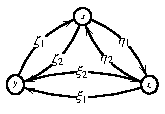
\includegraphics[width=0.68\textwidth]{figures/Fig_187_PDF296_Book284.pdf}
  \caption{三阶群作用下的 gentle 代数箭图（原书 p.284）}\label{fig:threefold-smash-quiver}
\end{figure}
\end{example}

覆盖方法可以为穿孔曲面构造带栈镜像。取有限阿贝尔群 $G$ 对 $\mathbb C^3$ 的对角作用。设对应的坐标特征标为 $\lambda_X,\lambda_Y,\lambda_Z\in\widehat G$，并满足
\[
  \lambda_X\lambda_Y\lambda_Z=1.
\]
此时函数 $XYZ$ 不变，所以它可以视为商栈 $[\mathbb C^3/G]$ 上的函数，并可考察相应矩阵分解。代数上，这些就是非交换 Landau--Ginzburg 模型 $(\mathbb C[X,Y,Z]\star G,XYZ)$ 的矩阵分解。

环 $B=\mathbb C[X,Y,Z]\star G$ 可以用一个箭图描述：顶点 $v_\phi$ 由 $\widehat G$ 编号，且有 $3|G|$ 条箭 $X_\phi,Y_\phi,Z_\phi$，分别连接 $v_\phi$ 与 $v_{\phi\lambda_X},v_{\phi\lambda_Y},v_{\phi\lambda_Z}$。这些箭之间的关系来自变量的交换关系：
\[
\begin{aligned}
  X_{\phi\lambda_Y}Y_\phi-Y_{\phi\lambda_X}X_\phi&=0,\\
  Y_{\phi\lambda_Z}Z_\phi-Z_{\phi\lambda_Y}Y_\phi&=0,\\
  Z_{\phi\lambda_X}X_\phi-X_{\phi\lambda_Z}Z_\phi&=0.
\end{aligned}
\]
正如每条箭在新箭图中有 $|G|$ 个对应物，标准矩阵分解 $M_X,M_Y,M_Z$ 也各有 $|G|$ 个版本。例如
\[
  M_{X_\phi}=\left(v_\phi B\oplus v_{\phi\lambda_X}B[1],
  \begin{pmatrix}
    0&Z_{\phi\lambda_Y\lambda_X}Y_{\phi\lambda_X}\\
    X_\phi&0
  \end{pmatrix}\right).
\]
基本态射 $\zeta_1\colon M_X\to M_Y$ 和 $\zeta_2\colon M_X\to M_Y$ 变为
\[
  \zeta_{1,\phi}\colon M_{X_\phi}\longrightarrow M_{Y_{\phi\lambda_Z}},
  \qquad
  \zeta_{2,\phi}\colon M_{Y_\phi}\longrightarrow M_{X_\phi}.
\]
% [Tutor Note: 原文把 $\zeta_1,\zeta_2$ 都写作 $M_X\to M_Y$，但紧接着的 $\zeta_{2,\phi}:M_{Y_\phi}\to M_{X_\phi}$ 方向相反；由上一节 $\mu(\zeta_1,\xi_1,\eta_1)=1_x$ 的循环结构，$\zeta_1,\zeta_2$ 中必有一个反向（原书 p.284 笔误），引用时以上标方向公式为准。]
这 $2|G|$ 个态射在箭图中组成 $|\widehat G/\langle\lambda_Z\rangle|$ 个环。

\begin{theorem}{阿贝尔商栈的镜像曲面}{abelian-stacky-pants-mirror}
若 $G\subset\mathrm{SL}_3(\mathbb C)$ 对 $\mathbb C^3$ 作对角作用，则
\[
  D^\pi\mathrm{MF}^{\pm}([\mathbb C^3/G],XYZ)
  \cong_\infty\mathrm{topFuk}^{\pm}(S,M),
\]
其中曲面 $S$ 的标记点数为
\[
  n=\frac{|G|}{|\langle\lambda_X\rangle|}
    +\frac{|G|}{|\langle\lambda_Y\rangle|}
    +\frac{|G|}{|\langle\lambda_Z\rangle|},
\]
其 Euler 示性数为 $n-|G|$。
\end{theorem}
\begin{proof}[证明思路]
与裤子曲面的情形相同，可以证明 $M_{X_\phi},M_{Y_\phi},M_{Z_\phi}$ 分裂生成 $D^\pi\mathrm{MF}^{\pm}([\mathbb C^3/G],XYZ)$。这些对象的自同态环是 $M_X\oplus M_Y\oplus M_Z$ 的自同态环与 $G$ 的叉积。由裤子曲面的镜像对称可知，这就是一个 gentle 代数与 $G$ 的叉积，也就是某个覆盖曲面的 gentle 代数。该曲面由 $2|G|$ 个三角形、$3|G|$ 条弧组成。其标记点数等于由 $\xi$、$\eta$ 或 $\zeta$ 组成的极小环路数；如上所见，这个数正是
\[
  n=\frac{|G|}{|\langle\lambda_X\rangle|}
    +\frac{|G|}{|\langle\lambda_Y\rangle|}
    +\frac{|G|}{|\langle\lambda_Z\rangle|}.
\]
\hfill$\square$
\end{proof}

\begin{example}[循环群作用的带栈镜像]\label{ex:cyclic-stacky-mirror}
令 $\mathbb Z_{2g+1}$ 以权重
\[
  \left(e^{2\pi i/(2g+1)},e^{2\pi i/(2g+1)},e^{-4\pi i/(2g+1)}\right)
\]
作用于 $\mathbb C[X,Y,Z]$。所得带栈 Landau--Ginzburg 模型的镜像是一个有三个标记点的曲面 $(S,M)$，其 Euler 示性数为 $3-(2g+1)=2-2g$，所以曲面亏格为 $g$。该曲面可以画成粘合在一起的 $2(2g+1)$ 边形：
\begin{figure}[H]\centering
  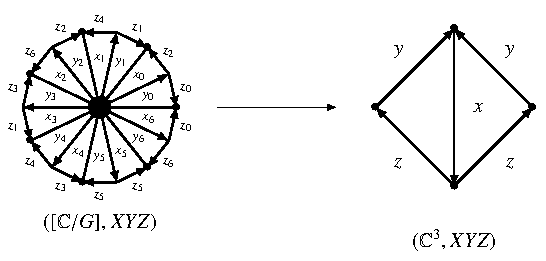
\includegraphics[width=0.9\textwidth]{figures/Fig_188_PDF297_Book285.pdf}
  \caption{循环群商栈及其裤子曲面镜像（原书 p.285）}\label{fig:cyclic-stacky-pants-mirror}
\end{figure}
\end{example}

\section{二聚体模型}\label{sec:dimer-models}
\takeaway{二聚体模型是弧系带循环定向的版本，镜面对偶在组合层面交换标记点与锯齿圈；Jacobi 代数 $(\mathrm{Jac}\,Q,\ell)$ 的矩阵分解的自同态环 $A_\infty$ 同构于 $\mathrm{Gtl}^{\pm}Q^\vee$，锯齿一致性保证这一镜像等价成立。}
我们可以把上述构造推广到其他非交换镜像。为此，先引入一些工具。

\begin{definition}{二聚体模型}{dimer-model}
二聚体模型\index{erjutimoxing@二聚体模型|hyperpage} $Q=(S,M,A)$ 由一个带标记曲面和一组剖分该曲面的弧组成，并要求每个多边形周围的弧都沿环形方向定向。把 $Q$ 看成嵌入曲面 $S$ 的箭图，其中 $Q_0=M$、$Q_1=A$。每个多边形给出 $Q$ 中的一个环路，把这些环路组成集合 $Q_2$。它是两个子集的并：$Q_2^+$ 由逆时针定向的环路组成，$Q_2^-$ 由顺时针定向的环路组成。
\end{definition}

\begin{note}\label{note:dimer-bipartite-origin}
二聚体模型的概念最初来自统计物理，原本指嵌入曲面的二分图\bookcite{137,132}。该图是弧系的对偶带状图：在每个顺时针多边形内放一个白点，在每个逆时针多边形内放一个黑点；相邻面的节点以边相连。
\end{note}

\begin{definition}{镜面（二聚体）对偶}{dimer-duality}
在二聚体模型集合上有一种对偶，称为镜面对偶\index{jingmianduiou@镜面对偶|hyperpage}\bookcite{121}或二聚体对偶\index{erjutiduiou@二聚体对偶|hyperpage}\bookcite{36,35}。其步骤如下：
\begin{enumerate}[label=(\roman*)]
  \item 沿弧把二聚体 $Q$ 切开；
  \item 翻转顺时针多边形中弧的定向；
  \item 按照相容的定向把所有部分重新粘合。
\end{enumerate}
所得新二聚体记为 $Q^\vee$。这一过程是对合，即 $Q^{\vee\vee}=Q$；$Q^\vee$ 也称为 $Q$ 的镜像二聚体\index{jingxiangerjuti@镜像二聚体|hyperpage}。
\end{definition}

\begin{example}[环面二聚体的对偶]\label{ex:torus-dimer-mirror}
从一个把环面剖分成两个三角形的二聚体出发，施行二聚体对偶后得到一个位于三标记球面上的二聚体：
\begin{figure}[H]\centering
  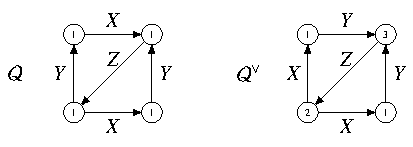
\includegraphics[width=0.66\textwidth]{figures/Fig_189_PDF298_Book286.pdf}
  \caption{环面二聚体及其镜像二聚体（原书 p.286）}\label{fig:torus-dimer-mirror}
\end{figure}
\end{example}

\begin{example}[更多二聚体对偶的例子]\label{ex:dimer-duality-examples}
下图给出文献\bookcite{36}中的另外四个例子。上排是四个二聚体：前两个嵌入环面，第三个嵌入亏格为 $2$ 的曲面，第四个位于球面。它们的镜像都嵌入环面，见下排。注意，前两个二聚体与其镜像同构，但这种同构并非显然。
\begin{figure}[H]\centering
  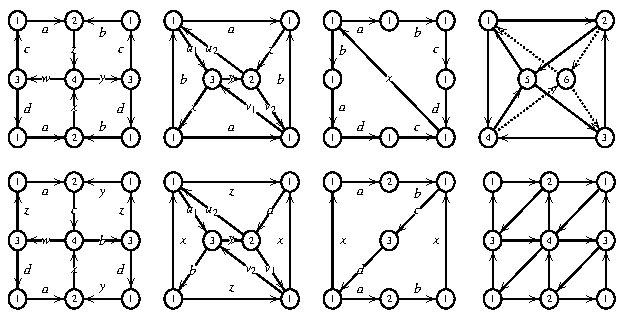
\includegraphics[width=0.99\textwidth]{figures/Fig_190_PDF299_Book287.pdf}
  \caption{四组二聚体及其镜像（原书 p.287）}\label{fig:four-dimer-duals}
\end{figure}
\end{example}

要记录二聚体对偶对亏格和标记点数的影响，需要引入锯齿路径\index{juchilujing@锯齿路径|hyperpage}的概念。

\begin{definition}{锯齿路径}{zigzag-path}
若路径 $a_1\cdots a_k$ 满足：当 $i$ 为偶数时，$a_i,a_{i+1}$ 在正向环路中相继出现；当 $i$ 为奇数时，它们在负向环路中相继出现，则称它为锯齿路径。换言之，这条路径在曲面上交替向左、向右转。从一条箭 $a$ 出发可以构造两条锯齿路径：锯齿射线先向左、再向右转；反锯齿射线先向右、再向左转。
\end{definition}

在对偶操作下，锯齿环路中的各条箭都会与镜像二聚体中的同一个标记点相接，因此二聚体对偶会交换标记点与锯齿环路：
\begin{figure}[H]\centering
  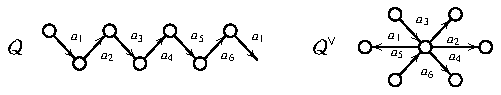
\includegraphics[width=0.64\textwidth]{figures/Fig_191_PDF299_Book287.pdf}
  \caption{锯齿路径及其在对偶二聚体中的表现（原书 p.287）}\label{fig:zigzag-path-duality}
\end{figure}

\begin{lemma}{二聚体对偶下的拓扑量}{dimer-duality-euler-characteristic}
设二聚体 $Q$ 有 $n$ 个标记点、$z$ 个锯齿环路，Euler 示性数为 $\chi$。则 $Q^\vee$ 有 $z$ 个标记点、$n$ 个锯齿环路，Euler 示性数为 $\chi-n+z$。
\end{lemma}

\begin{definition}{Jacobi 代数}{jacobi-algebra}
对二聚体 $Q$，可以构造一个非交换代数，称为它的 Jacobi 代数\index{jacobidaishu@Jacobi 代数|hyperpage}。它是箭图 $Q$ 的路径代数除以如下关系：对每条箭 $a$，令 $a\ell_a$ 和 $ar_a$ 是 $Q_2$ 中包含 $a$ 的两个环路，则令两条回路路径相等：
\[
  \mathrm{Jac}\,Q:=
  \frac{\mathbb C Q}{\langle \ell_a-r_a\mid a\in Q_1,\;a\ell_a\in Q_2^+,\;ar_a\in Q_2^-\rangle}.
\]
\begin{figure}[H]\centering
  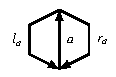
\includegraphics[width=0.42\textwidth]{figures/Fig_192_PDF299_Book287.pdf}
  \caption{一条箭及其所在的正、负向环路（原书 p.287）}\label{fig:dimer-jacobi-relation}
\end{figure}
这些关系表示：对每条箭，沿左侧环路返回与沿右侧环路返回，在代数中是相同的路径。
\end{definition}

\begin{lemma}{Jacobi 代数的中心元}{jacobi-central-element}
Jacobi 代数 $\mathrm{Jac}\,Q$ 含有一个中心元 $\ell$，并且对每个 $v\in Q_0$，$v\ell$ 都是 $Q_2$ 中的一个环路。
\end{lemma}
\begin{proof}[证明思路]
对每个 $v$，取一个从 $v$ 出发且代表 $Q_2$ 中环路的闭路 $\ell_v$。由于 Jacobi 关系，$\ell_v$ 在 $\mathrm{Jac}\,Q$ 中不依赖于闭路的具体选择。进一步，对任意路径 $p$，利用这些关系可得
\[
  \ell_{h(p)}p=p\ell_{t(p)}.
\]
因此 $\ell:=\sum_{v\in Q_0}\ell_v$ 是中心元。\hfill$\square$
\end{proof}

\begin{definition}{二聚体的 Landau--Ginzburg 模型}{dimer-landau-ginzburg}
二聚体 $Q$ 的 Landau--Ginzburg 模型\index{qdelandauginzburgmoxing@Q 的 Landau–Ginzburg 模型|hyperpage}是二元组 $(\mathrm{Jac}\,Q,\ell)$。
\end{definition}

\begin{example}[裤子曲面的 Jacobi 代数]
从例\ref{ex:torus-dimer-mirror} 中把环面剖分成两个三角形的二聚体 $Q$ 出发。其 Jacobi 代数是三元多项式环
\[
  \mathrm{Jac}\,Q=
  \frac{\mathbb C\langle X,Y,Z\rangle}
       {\langle XY-YX,\;XZ-ZX,\;YZ-ZY\rangle},
\]
中心元为 $\ell=XYZ$。它的 Landau--Ginzburg 模型是裤子曲面的镜像，因此 $Q^\vee$ 位于一个有三个标记点的球面上。
\end{example}
% [Tutor Note: 直觉上，二聚体对偶就是镜像对称的组合版本：A 侧的弧系与 B 侧 Jacobi 代数的矩阵分解互为镜像，锯齿圈（箭的极大交替路径）在对偶下变成标记点，这正是亏格与标记点数在对偶下互换的来源。]

这一构造也与覆盖相容。先考虑有一个穿孔的环面，并通过选取两个向量 $v_1,v_2\in\mathbb Z^2$ 来扩大其基本区域，令
\[
  S=\mathbb R^2/(\mathbb Z v_1+\mathbb Z v_2).
\]
取格点集 $M=\mathbb Z^2/(\mathbb Z v_1+\mathbb Z v_2)$ 作为标记点，\linebreak[3] 并取从每个标记点出发、方向向量分别为\linebreak $(1,0),(0,1),(-1,-1)$ 的箭组成弧系。对每个 $m\in M$，按方向把这些箭记为 $x_m,y_m,z_m$。总共有 $k=|\det(v_1,v_2)|$ 个标记点和 $3k$ 条箭，它们把环面剖分成 $2k$ 个三角形。把这个二聚体记为 $Q_{v_1,v_2}$。

注意，$M=\mathbb Z^2/(\mathbb Z v_1+\mathbb Z v_2)$ 本身也是一个群。令 $G=\mathrm{Hom}(M,\mathbb C^*)$，则 $M$ 是 $G$ 的特征群。可以定义 $G$ 在 $\mathbb C[X,Y,Z]$ 上的作用：
\[
  g\cdot X=g(1,0)X,\qquad
  g\cdot Y=g(0,1)Y,\qquad
  g\cdot Z=g(-1,-1)Z.
\]
这里 $(1,0),(0,1),(-1,-1)$ 都视为 $M$ 的元素，因此可以将 $g\in G=\mathrm{Hom}(M,\mathbb C^*)$ 作用于它们。

\begin{lemma}{覆盖环面二聚体的 Jacobi 代数}{cover-dimer-jacobi-algebra}
二聚体 $Q_{v_1,v_2}$ 的 Jacobi 代数同构于
\[
  \mathrm{Jac}\,Q_{v_1,v_2}\cong\mathbb C[X,Y,Z]\star G.
\]
\end{lemma}
\begin{proof}
代数 $\mathbb C[X,Y,Z]\star G$ 的箭图顶点是 $G$ 的特征，因而与 $M$ 中元素对应。其箭形如 $X_\phi,Y_\phi,Z_\phi$，其中 $\phi\in\widehat G$，自然对应于 $x_m,y_m,z_m$。因此存在自然满射
\[
  \mathbb C Q\longrightarrow\mathbb C[X,Y,Z]\star G.
\]
该映射通过 Jacobi 代数，因为 $\mathrm{Jac}\,Q$ 中的关系都形如 $x_\phi y_\psi-y_\phi x_\psi$（或把 $\{x,y,z\}$ 中其他两种变量配对得到的关系）；在映射下，这些关系变成 $[X,Y]e_\psi=0$。

Jacobi 代数中的关系说明，每条路径都由其起点与其中 $x,y,z$ 的数目唯一确定。因此，没有两条不同路径会映到 $\mathbb C[X,Y,Z]\star G$ 中的同一个元素，故上述映射也是单射。\hfill$\square$
\end{proof}

若把这些带栈 Landau--Ginzburg 模型视为非交换 Landau--Ginzburg 模型，就可以把镜像对称解释为二聚体对偶的一种实例。箭图 $Q=Q_{v_1,v_2}$ 中每条箭 $a$ 都自然对应于 $\ell\in\mathrm{Jac}\,Q$ 的一个矩阵分解：
\begin{figure}[H]\centering
  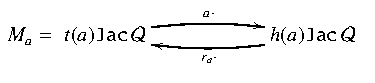
\includegraphics[width=0.38\textwidth]{figures/Fig_193_PDF301_Book289.pdf}
  \caption{由箭构造的 Jacobi 代数矩阵分解（原书 p.289）}\label{fig:arrow-matrix-factorization}
\end{figure}
由定理\ref{thm:abelian-stacky-pants-mirror}可知，矩阵分解 $M_a$ 的直和的自同态环 $A_\infty$ 同构于某个曲面弧系的 gentle 代数。直接计算可见，该弧系恰是镜像二聚体 $Q^\vee$ 所对应的弧系：
\[
  \mathrm{End}_{\mathrm{MF}^{\pm}(\mathrm{Jac}\,Q,\ell)}
  \left(\bigoplus_{a\in Q_1}M_a\right)
  \cong_\infty\mathrm{Gtl}^{\pm}Q^\vee.
\]

\begin{example}[环面覆盖与二聚体对偶]\label{ex:cyclic-dimer-duality}
令 $v_1=(g+1,g)$、$v_2=(g,g+1)$。此时
\[
  M=\mathbb Z^2/(\mathbb Z v_1+\mathbb Z v_2)
  \cong\mathbb Z/(2g+1)\mathbb Z=\langle(1,1)\rangle.
\]
取对偶生成元 $u\in\mathrm{Hom}(M,\mathbb C^*)$，令它把 $(1,1)$ 映到 $e^{2\pi i/(2g+1)}$。于是
\[
  u\cdot X=e^{2\pi i/(2g+1)}X,\qquad
  u\cdot Y=e^{2\pi i/(2g+1)}Y,\qquad
  u\cdot Z=e^{-4\pi i/(2g+1)}Z.
\]
\begin{figure}[H]\centering
  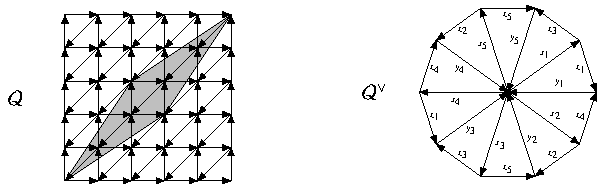
\includegraphics[width=0.86\textwidth]{figures/Fig_194_PDF301_Book289.pdf}
  \caption{互为镜像的两个环面二聚体（原书 p.289）}\label{fig:cyclic-dimer-dual}
\end{figure}
从二聚体角度看，$Q$ 的亏格为 $1$、有 $2g+1$ 个标记点；其对偶二聚体 $Q^\vee$ 的亏格为 $g$、有 $3$ 个标记点。这与例\ref{ex:cyclic-stacky-mirror}相同。
\end{example}

从这个例子可能会猜想，任意二聚体都具有这样的二聚体对偶性质；遗憾的是，并非如此。关键问题在于某些情形下 Jacobi 代数的性质不够好（例如整体维数不是有限的），因此必须给二聚体附加一些一致性条件\index{yizhixingtiaojian@一致性条件|hyperpage}。文献中研究过多种一致性条件\bookcite{180,63,42,126,33}；下面聚焦其中一个。

\begin{definition}{锯齿一致二聚体}{zigzag-consistent-dimer}
若对 $Q_1$ 中每条箭 $a$，锯齿射线与反锯齿射线在万有覆盖中除 $a$ 本身外不相交，则称二聚体 $Q$ 是锯齿一致\index{juchiyizhixing@锯齿一致性|hyperpage}的。
\end{definition}

\begin{example}[二聚体的一致性]
下表列出例\ref{ex:dimer-duality-examples}中八个二聚体的一致性性质：
\[
\begin{array}{c|cccc}
 &Q_1&Q_2&Q_3&Q_4\\\hline
\text{锯齿一致}&\text{是}&\text{否}&\text{是}&\text{否}\\
\text{镜像一致}&\text{是}&\text{否}&\text{否}&\text{是}
\end{array}
\]
对上排第二个二聚体，可以直接检查从 $z$ 出发的锯齿射线和反锯齿射线也会在 $x$ 处相交。
\end{example}

\begin{theorem}{锯齿一致二聚体的镜像等价}{zigzag-consistent-dimer-mirror}
若二聚体 $Q$ 锯齿一致，则
\[
  \mathrm{End}_{\mathrm{MF}^{\pm}(\mathrm{Jac}\,Q,\ell)}
  \left(\bigoplus_{a\in Q_1}M_a\right)
  \cong_\infty\mathrm{Gtl}^{\pm}Q^\vee.
\]
\end{theorem}
\begin{proof}[证明思路]
设 $M_a,M_b$ 是分别来自箭 $a,b$ 的两个矩阵分解，且 $ax_1\cdots x_kb$ 是一条锯齿路径。可以利用这条锯齿路径的反向路径构造一个从 $M_a$ 到 $M_b$ 的态射。这两条路径 $z^+,z^-$ 分别沿着锯齿路径两侧的正向环和负向环返回：
\begin{figure}[H]\centering
  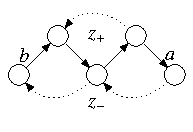
\includegraphics[width=0.48\textwidth]{figures/Fig_195_PDF302_Book290.pdf}
  \caption{锯齿路径两侧的正、负向回路（原书 p.290）}\label{fig:zigzag-positive-negative-paths}
\end{figure}
该态射的形状如下：
\begin{figure}[H]\centering
  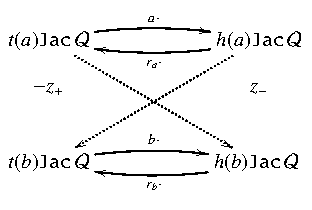
\includegraphics[width=0.58\textwidth]{figures/Fig_196_PDF302_Book290.pdf}
  \caption{由锯齿路径给出的矩阵分解态射（原书 p.290）}\label{fig:zigzag-mf-morphism}
\end{figure}
在二聚体对偶构造下，锯齿环路变成 $Q^\vee$ 中的标记点，而锯齿路径可视为绕这些标记点转向的角，换言之，就是 gentle 代数 $\mathrm{Gtl}^{\pm}Q^\vee$ 中的路径。若 $Q$ 锯齿一致，可以证明这一解释延拓为\linebreak $\mathrm{End}_{\mathrm{MF}^{\pm}(\mathrm{Jac}\,Q,\ell)}(\bigoplus_{a\in Q_1}M_a)$ 与 $\mathrm{Gtl}^{\pm}Q^\vee$ 之间的 $A_\infty$ 同构。证明的更多细节见\bookcite{36}。\hfill$\square$
\end{proof}

\begin{example}[两个正方形铺砌的环面]\label{ex:two-square-dimer}
取一个有两个标记点的环面，并用两个正方形铺砌。其对偶二聚体是有四个标记点的球面。容易验证，第一个二聚体是一致的：在万有覆盖中，锯齿射线是沿不同方向延伸的阶梯线，所以只能在一条箭上相交。第二个二聚体不一致，因为它位于球面上，锯齿射线总会多次相交。
\begin{figure}[H]\centering
  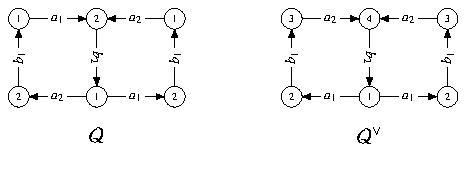
\includegraphics[width=0.86\textwidth]{figures/Fig_197_PDF303_Book291.pdf}
  \caption{环面上的二聚体及球面上的镜像二聚体（原书 p.291）}\label{fig:two-square-dimer-dual}
\end{figure}
其 Jacobi 代数为
\[
  \mathrm{Jac}\,Q:=
  \frac{\mathbb C\langle a_1,a_2,b_1,b_2\rangle}{I},
\]
其中 $I$ 由下列四个关系生成：
\[
\begin{aligned}
  a_1b_1a_2-a_2b_1a_1,&\qquad a_1b_2a_2-a_2b_2a_1,\\
  b_1a_1b_2-b_2a_1b_1,&\qquad b_1a_2b_2-b_2a_2b_1.
\end{aligned}
\]
中心元为 $\ell=a_1b_1a_2b_2+b_1a_2b_2a_1$。非交换 Landau--Ginzburg 模型 $(\mathrm{Jac}\,Q,\ell)$ 是四标记球面的镜像。
\begin{figure}[H]\centering
  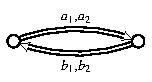
\includegraphics[width=0.43\textwidth]{figures/Fig_198_PDF303_Book291.pdf}
  \caption{构成 Jacobi 关系的两组平行箭（原书 p.291）}\label{fig:two-square-jacobi-arrows}
\end{figure}

正如裤子曲面的镜像是嵌入光滑三维空间 $\mathbb A^3$ 中的 Landau--Ginzburg 模型，这些 Jacobi 代数也应被视为非交换空间。若二聚体 $Q$ 一致且其曲面是环面，则 $\mathrm{Jac}\,Q$ 实际上与一个真正的交换空间——三维环簇 Calabi--Yau 簇——导出等价。该簇的 Newton 多边形各边的法向量，与二聚体万有覆盖中锯齿射线的方向一一对应（在万有覆盖中作图时，基本区域取为单位正方形）。关于三维环簇 Calabi--Yau 簇和二聚体模型的更多关系，见\bookcite{125,127,179}。
\end{example}

\begin{example}[三标记环面二聚体的镜像]\label{ex:five-zigzag-dimer}
取文献\bookcite{35}中的二聚体 $Q$。它嵌入有三个标记点的环面，而其镜像二聚体 $Q^\vee$ 位于有五个标记点的球面。
\begin{figure}[H]\centering
  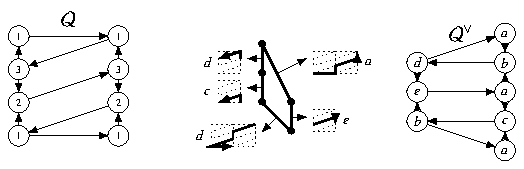
\includegraphics[width=0.94\textwidth]{figures/Fig_199_PDF304_Book292.pdf}
  \caption{环面二聚体、其镜像及 Newton 多边形（原书 p.292）}\label{fig:five-zigzag-dimer}
\end{figure}
二聚体 $Q$ 有五条锯齿路径，图中央画出了 Newton 多边形 $\square$，其边垂直于这些锯齿路径。Jacobi 代数 $\mathrm{Jac}\,Q$ 与第\ref{subsec:one-two-three-models}节中的三维环簇 $X^3_{\boxtimes}$ 导出等价。
\end{example}

\section{众多镜像}\label{sec:mirrors-galore}
\takeaway{同一带标记曲面可有三类镜像：Newton 多边形三角剖分给出的三维环簇、$[\mathbb C^3/G]$ 型的带栈 Landau--Ginzburg 模型，与锯齿一致二聚体给出的非交换 Landau--Ginzburg 模型；亏格与标记点数由多边形或二聚体的组合量算出。}
设 $(S,M)$ 是亏格为 $g$、有 $n$ 个内部标记点的带标记曲面。可以为它构造若干不同类型的镜像；每一类镜像也会因额外的组合数据而有不同选择。

\begin{itemize}
  \item \textbf{交换 Landau--Ginzburg 模型。}对 Newton 多边形作三角剖分，可以构造一个三维环簇 $X_{\boxtimes}^{3}$ 及其上的全局函数 $\ell$，并得到
  \[
    \mathrm{topFuk}^{\pm}(S,M)\simeq D^{\pi}\mathrm{MF}^{\pm}(X_{\boxtimes}^{3},\ell).
  \]
  曲面的标记点数等于多边形边界格点数，亏格等于多边形内部格点数。

  \item \textbf{带栈 Landau--Ginzburg 模型。}取有限阿贝尔群 $G\subset\mathrm{SL}_3(\mathbb C)$，可构造三维商栈 $[\mathbb C^3/G]$ 及其不变函数 $\ell=XYZ$，并有
  \[
    \mathrm{topFuk}^{\pm}(S,M)\simeq D^{\pi}\mathrm{MF}^{\pm}([\mathbb C^3/G],\ell).
  \]
  标记点数等于 $X,Y,Z$ 三个函数的稳定子群阶数之和，即
  \[
    n=|G_X|+|G_Y|+|G_Z|,
  \]
  而曲面的亏格为
  \[
    g=\frac12\bigl(|G|-|G_X|-|G_Y|-|G_Z|\bigr)+1.
  \]

  \item \textbf{非交换 Landau--Ginzburg 模型。}取一个锯齿一致的二聚体模型 $Q$，它给出 Jacobi 代数 $\mathrm{Jac}\,Q$ 及其中心元 $\ell$。每条箭 $a\in Q_1$ 对应于 $(\mathrm{Jac}\,Q,\ell)$ 的一个矩阵分解 $M_a$，也对应于镜像二聚体 $Q^{\vee}$ 中的一条弧 $a$，从而给出 $\mathrm{topFuk}^{\pm}(S,M)$ 中的对象 $L_a$。两侧的生成子范畴之间有 $A_{\infty}$ 同构：
  \[
    D^{\pi}\mathrm{MF}^{\pm}(\mathrm{Jac}\,Q,\ell)\supset
    \langle M_a\mid a\in Q_1\rangle
    \cong_\infty
    \langle L_a\mid a\in Q^{\vee}_1\rangle
    \subset\mathrm{topFuk}^{\pm}(S,M).
  \]
  曲面的标记点数 $n$ 等于 $Q$ 的锯齿环路数，曲面亏格为
  \[
    g=\frac12\bigl(\#Q_1-\#Q_2-n\bigr)+1.
  \]
\end{itemize}

\section{习题}\label{sec:gluing-exercises}

\begin{exercise}\label{exer:gluing-min-arcs}
设 $(S,M)$ 是亏格为 $g$ 的带标记曲面，有 $m$ 个边界分支，第 $i$ 个边界分支上有 $b_i$ 个标记点（$1\le i\le m$），并有 $k$ 个内部标记点。写出将曲面剖分所需弧数的最小值公式。
\end{exercise}

\begin{exercise}\label{exer:gluing-linear-quiver-surface}
找一个曲面及其弧系，使相应 gentle 代数是下图箭图的路径代数：
\begin{figure}[H]\centering
  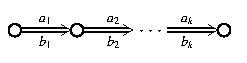
\includegraphics[width=0.43\textwidth]{figures/Fig_200_PDF305_Book293.pdf}
  \caption{练习 9.2 中的箭图（原书 p.293）}
\end{figure}
其关系为 $a_{i+1}a_i=b_{i+1}b_i=0$，且所有箭的次数均为 $0$。用 $k$ 表示该曲面的亏格和边界分支数。
\end{exercise}

\begin{exercise}\label{exer:gluing-self-intersecting-string}
设曲线 $\gamma$ 从两个不同的标记点出发，并自交一次，围成一个不可缩的环。确定相应弦对象在 $D\mathrm{Gtl}^{\pm}A$ 中的自同态环。
\end{exercise}

\begin{exercise}\label{exer:gluing-polygon-hocolim}
取一个多边形并将其三角剖分。利用这一三角剖分，把多边形的 Fukaya 范畴写成若干个下图所示范畴的同伦余极限：
\begin{figure}[H]\centering
  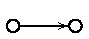
\includegraphics[width=0.28\textwidth]{figures/Fig_201_PDF305_Book293.pdf}
  \caption{练习 9.4 中的基本箭图范畴（原书 p.293）}
\end{figure}
\end{exercise}

\begin{exercise}\label{exer:gluing-cylinder-two-marks}
将例\ref{ex:cylinder-tubular-gluing}推广到圆柱两侧各有两个标记点的情形，并完成相应构造。
\end{exercise}

\begin{exercise}\label{exer:gluing-local-p2}
考虑由 $(1,0,1)$、$(0,1,1)$ 和 $(-1,-1,1)$ 张成的多边形，并通过从顶点连接到 $v_0=(0,0,1)$ 来三角剖分。相应的光滑三维簇 $X_{\boxtimes}^{3}$ 是 $\mathbb P^2$ 的反典范线丛全空间；令 $D=\mathbb P^2$ 为对应于 $v_0$ 的除子。
\begin{enumerate}[label=(\roman*)]
  \item 确定与 $(X_{\boxtimes}^{3},\ell)$ 镜像的曲面 $S_{g,n}$ 的亏格和穿孔数。
  \item 在下列识别下，求出与结构层 $\mathcal O_D$ 的像相对应的 $\ell$ 的矩阵分解 $M$：
  \[
    \mathrm{MF}^{\pm}(X_{\boxtimes}^{3},\ell)
    =D_{\mathrm{Sing}}\bigl(\ell^{-1}(0)\bigr)
    =\frac{D\mathrm{Coh}\bigl(\ell^{-1}(0)\bigr)}
    {\mathrm{Perf}\bigl(\ell^{-1}(0)\bigr)}.
  \]
  提示：把 $\mathrm{MF}^{\pm}(\mathbb C^3,XYZ)$ 中形如 $M_X$ 的矩阵分解粘合起来。
  \item 利用同伦极限的解释，确定曲面 $S_{g,n}$ 上与 $M$ 对应的曲线。
\end{enumerate}
\end{exercise}

\begin{exercise}\label{exer:gluing-smash-product}
验证有限群对 $A_{\infty}$ 代数的作用所定义的叉积 $A\mathbin{\star}G$，按定义\ref{def:ainfty-smash-product} 的构造仍是一个 $A_{\infty}$ 代数。
\end{exercise}

\begin{exercise}\label{exer:gluing-klein-stacky-mirror}
令 $G=\mathbb Z_2\times\mathbb Z_2$ 作用于 $\mathbb C^3$，作用为
\[
  (a,b)\cdot(X,Y,Z)=\bigl((-1)^aX,(-1)^bY,(-1)^{a+b}Z\bigr).
\]
求带栈 Landau--Ginzburg 模型 $([\mathbb C^3/G],XYZ)$ 的镜像，并将其描述为三穿孔球面上的覆盖。同时，给出满足 $\mathrm{Jac}\,Q\cong\mathbb C[X,Y,Z]\mathbin{\star}G$ 的二聚体模型 $Q$。
\end{exercise}

\begin{exercise}\label{exer:gluing-dimer-mutation}
设 $Q$ 是锯齿一致的二聚体模型，$v\in Q_0$ 是一个顶点，有两条箭 $a_1,a_2$ 指向 $v$，另有两条箭 $b_1,b_2$ 从 $v$ 指出。通过反转这些箭并为路径 $b_i a_j$ 加入新箭来变异顶点，最后删去所有二环。局部变异如下图所示：
\begin{figure}[H]\centering
  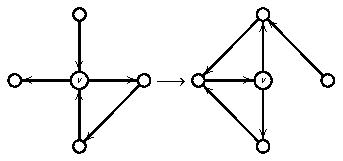
\includegraphics[width=0.46\textwidth]{figures/Fig_202_PDF306_Book294.pdf}
  \caption{二聚体模型的顶点变异（原书 p.294）}
\end{figure}
证明变异后的二聚体模型 $\mu_v Q$ 仍然锯齿一致。
\end{exercise}

\begin{exercise}\label{exer:gluing-z3-dimer}
令 $G=\mathbb Z_3=\langle g\mid g^3=1\rangle$ 作用于 $\mathbb C^3$，且
\[
  g\cdot(X,Y,Z)=\bigl(e^{2\pi i/3}X,e^{2\pi i/3}Y,e^{2\pi i/3}Z\bigr).
\]
代数 $\mathbb C[X,Y,Z]\mathbin{\star}G$ 可表示为带关系的下图箭图：
\begin{figure}[H]\centering
  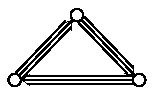
\includegraphics[width=0.4\textwidth]{figures/Fig_203_PDF306_Book294.pdf}
  \caption{练习 9.10 中的箭图（原书 p.294）}
\end{figure}
\begin{enumerate}[label=(\roman*)]
  \item 把 $Q$ 画成环面上的二聚体模型，使得 $\mathrm{Jac}\,Q\cong\mathbb C[X,Y,Z]\mathbin{\star}G$。
  \item 证明维数向量 $\alpha=(1,1,1)$、稳定参数 $\theta=(-2,1,1)$ 对应的模空间 $M_\theta(\mathrm{Jac}\,Q,\alpha)$ 同构于习题\ref{exer:gluing-local-p2} 中的簇。
  \item 求一个矩阵分解 $M$，使其对应于中心 $\mathbb P^2$ 的结构层。
\end{enumerate}
\end{exercise}

\chapterreview{%
\textbf{全章地位。}本章是全书构造的中枢。它用带标记曲面与生成弧系把曲面的 partially wrapped Fukaya 范畴完全组合化，得到只依赖多边形剖分的 $\mathrm{topFuk}^{\pm}(S,M)$，同时把 Kontsevich 关于“wrapped Fukaya 范畴是拉格朗日骨架上的范畴层”的设想在一维情形下兑现。此前的 gentle 代数、矩阵分解与二聚体在此合流，此后的分次版本、稳定性与变形都以本章的模型为出发点。

\textbf{知识脉络。}带标记曲面 $\to$ 生成弧系 $\to$ 箭图 $Q_A$ 与 gentle $A_\infty$ 代数 $\mathrm{Gtl}^{\pm}A$（面状路径置零，闭多边形贡献高阶乘积）$\to$ 换弧不变性（扭曲完备化与 Hatcher 翻转）$\to$ 定义 $\mathrm{topFuk}^{\pm}:=D\mathrm{Gtl}^{\pm}A$ $\to$ 用弧与角缝合曲线，得弦对象与带对象（交点为态射，多边形计数乘积）$\to$ 沿带状图（协变余层、同伦余极限）与管状图（反变层、同伦极限）粘合 $\to$ 以裤子曲面为基本构件做镜像并粘出高亏格曲面 $\to$ 覆盖与叉积 $A\star G$ $\to$ 二聚体与 Jacobi 代数。主线是“局部可算、整体靠粘合”。

\textbf{核心结论。}（1）$\mathrm{topFuk}^{\pm}(S,M)=D\mathrm{Gtl}^{\pm}A$ 与弧系无关；换弧归结为把反向弧识别为 $a[1]$，再由 Hatcher 定理化为四边形的对角翻转。（2）开曲线的同伦类实现为弦对象，闭曲线连同绕行变换实现为带对象 $B(L,T^\lambda)$；带对象间的态射由交点给出，乘积由曲线围成的浸入多边形计数，这正是 Fukaya 范畴的组合影子。（3）沿带状图的 $R$ 是余层，同伦余极限还原整体范畴；沿管状图的 $T$ 是层，同伦极限（须先取 ind-完备化）还原整体范畴。（4）裤子曲面 $\mathrm{topFuk}^{\pm}\cong_\infty\mathrm{MF}^{\pm}(\mathbb C^3,XYZ)$，粘合与矩阵分解的 Čech 型粘合逐项对应，得 $\mathrm{MF}^{\pm}(Y_T,\ell)\cong_\infty\mathrm{topFuk}^{\pm}(\Sigma_T)$，其中亏格等于多边形内部格点数、标记点数等于边界格点数。（5）覆盖拉回对应叉积 $A\star G\cong\mathrm{Gtl}^{\pm}\widetilde A$，据此算出带栈镜像的标记点数 $n=\sum_i|G|/|\langle\lambda_i\rangle|$。（6）锯齿一致二聚体满足 $\operatorname{End}(\bigoplus_aM_a)\cong_\infty\mathrm{Gtl}^{\pm}Q^\vee$。

\textbf{辨析与提醒。}其一，本章的等价都是 $A_\infty$ 等价而非严格同构；极小模型中的乘积依赖标记弧（引理 9.10 给出两种取值），只在 $A_\infty$ 同构意义下良定，不能把某一模型算出的数值当作不变量。其二，闭多边形产生非零高阶乘积、内部标记点使代数无限维，这是两件独立的事；例 9.2 的圆盘既有内部标记点又无高阶乘积，正可对照。其三，文献约定差别很大：有的挖去标记点，有的把非标记边界段压成 stop；对照公式前须先确认 $(S,M)$ 取哪一种。其四，带对象允许非平凡绕行变换，而弦对象的局部系统总可化为平凡，这一区别到第 12 章填充标记点时才显出作用。

\textbf{评注。}作者用一维曲面换取“一切可组合计算”，代价是几乎不出现 Floer 理论，也不处理 $\mathbb Z$ 分次与圆盘泡。第 9.2 节关于极小模型依赖的处理值得细读：作者用标记弧点破了良定性问题，却未系统展开“乘法依赖模型”的一般理论，想深究的读者应回到 Haiden--Katzarkov--Kontsevich 与 Pascaleff--Sibilla 的原文。二聚体一节密度最高：Jacobi 代数、锯齿一致性与镜像等价三者串联，实际上已经预告了第 11 章的环簇消解与第 12 章的填充构造。阅读建议：先抓住“弧—曲线—对象”这本词典，再把粘合理解为范畴层的层论操作，最后用二聚体检验自己是否真的会算乘积。}
